%% 由 build/emit_tex.py 生成（生成物，勿手改）；定制请放 user_style.tex / user_meta.yaml
\chapter{第 6 章 ·
Networkx及其基本使用}\label{ux7b2c-6-ux7ae0-networkxux53caux5176ux57faux672cux4f7fux7528}

\section{01
创建图：无向图、有向图、属性与生成器}\label{ux521bux5efaux56feux65e0ux5411ux56feux6709ux5411ux56feux5c5eux6027ux4e0eux751fux6210ux5668}

\begin{quote}
本节对应原版 6.1 的内容，并增补学习目标、常见误区、思考题与延伸阅读。
配套图：figures/06-networkx/graph\_basic.png（由
build/make\_chap6\_figures.py 生成）。
\end{quote}

\subsection{本节目标}\label{ux672cux8282ux76eeux6807-23}

\begin{itemize}
\tightlist
\item
  理解 NetworkX 中图对象（Graph / DiGraph）的基本概念；
\item
  会创建空图并添加节点、边；
\item
  会读取 nodes / edges / degree，访问邻居、前驱、后继与入度/出度；
\item
  会给节点和边添加属性（权重、标签）；
\item
  会用常用图生成器（path\_graph、cycle\_graph、complete\_graph、grid\_2d\_graph、karate\_club\_graph
  等）快速造图；
\item
  会用 nx.to\_numpy\_array 把图转成邻接矩阵，供 NumPy 使用。
\end{itemize}

\subsection{先修}\label{ux5148ux4fee-16}

\begin{itemize}
\tightlist
\item
  Python 列表、元组、字典、for 循环；了解函数与类的基本概念。
\end{itemize}

\begin{center}\rule{0.5\linewidth}{0.5pt}\end{center}

\subsection{1.1 NetworkX
简介与安装}\label{networkx-ux7b80ux4ecbux4e0eux5b89ux88c5}

NetworkX 是 Python 生态中创建、操作、分析复杂网络的库。它是一个纯 Python
实现（底层可结合 NumPy/SciPy），接口直观，覆盖图论与网络科学的常用算法。

安装（建议 Python 3.10+）：

\begin{Shaded}
\begin{Highlighting}[]
\ExtensionTok{pip}\NormalTok{ install networkx}
\end{Highlighting}
\end{Shaded}

导入并查看版本：

\begin{Shaded}
\begin{Highlighting}[]
\ImportTok{import}\NormalTok{ networkx }\ImportTok{as}\NormalTok{ nx}
\BuiltInTok{print}\NormalTok{(nx.\_\_version\_\_)}
\end{Highlighting}
\end{Shaded}

\begin{Shaded}
\begin{Highlighting}[]
\NormalTok{3.3}
\end{Highlighting}
\end{Shaded}

\begin{quote}
说明：本章代码在 NetworkX 3.x
下验证；不同小版本的个别函数参数可能变化，遇到不熟悉的接口请以官方文档为准。
\end{quote}

\begin{center}\rule{0.5\linewidth}{0.5pt}\end{center}

\subsection{1.2
创建无向图（Graph）}\label{ux521bux5efaux65e0ux5411ux56fegraph}

无向图的边没有方向，用 nx.Graph 创建。

\begin{Shaded}
\begin{Highlighting}[]
\ImportTok{import}\NormalTok{ networkx }\ImportTok{as}\NormalTok{ nx}

\CommentTok{\#\# 创建一个空的无向图}
\NormalTok{G }\OperatorTok{=}\NormalTok{ nx.Graph()}

\CommentTok{\#\# 添加节点}
\NormalTok{G.add\_node(}\DecValTok{1}\NormalTok{)}
\NormalTok{G.add\_nodes\_from([}\DecValTok{2}\NormalTok{, }\DecValTok{3}\NormalTok{, }\DecValTok{4}\NormalTok{])}

\CommentTok{\#\# 添加边}
\NormalTok{G.add\_edge(}\DecValTok{1}\NormalTok{, }\DecValTok{2}\NormalTok{)}
\NormalTok{G.add\_edges\_from([(}\DecValTok{2}\NormalTok{, }\DecValTok{3}\NormalTok{), (}\DecValTok{3}\NormalTok{, }\DecValTok{4}\NormalTok{), (}\DecValTok{4}\NormalTok{, }\DecValTok{1}\NormalTok{)])}

\CommentTok{\#\# 查看节点与边}
\BuiltInTok{print}\NormalTok{(G.nodes())}
\BuiltInTok{print}\NormalTok{(G.edges())}
\end{Highlighting}
\end{Shaded}

\begin{Shaded}
\begin{Highlighting}[]
\NormalTok{[1, 2, 3, 4]}
\NormalTok{[(1, 2), (1, 4), (2, 3), (3, 4)]}
\end{Highlighting}
\end{Shaded}

说明：add\_node 加单个节点；add\_nodes\_from
加一个可迭代集合（列表、元组、range）；add\_edge
加单条边；add\_edges\_from 加多条边。G.nodes() 与 G.edges()
返回的是视图对象，可转成 list / tuple 使用。

\subsubsection{1.2.1
度（Degree）与邻居}\label{ux5ea6degreeux4e0eux90bbux5c45}

无向图中，节点的度是与它相连的边数。

\begin{Shaded}
\begin{Highlighting}[]
\BuiltInTok{print}\NormalTok{(G.degree())                 }\CommentTok{\# 所有节点的度}
\ControlFlowTok{for}\NormalTok{ node, degree }\KeywordTok{in}\NormalTok{ G.degree():}
    \BuiltInTok{print}\NormalTok{(}\SpecialStringTok{f"Node }\SpecialCharTok{\{}\NormalTok{node}\SpecialCharTok{\}}\SpecialStringTok{ has degree }\SpecialCharTok{\{}\NormalTok{degree}\SpecialCharTok{\}}\SpecialStringTok{"}\NormalTok{)}
\BuiltInTok{print}\NormalTok{(}\BuiltInTok{list}\NormalTok{(G.neighbors(}\DecValTok{1}\NormalTok{)))       }\CommentTok{\# 节点 1 的所有邻居}
\end{Highlighting}
\end{Shaded}

\begin{Shaded}
\begin{Highlighting}[]
\NormalTok{[(1, 2), (2, 2), (3, 2), (4, 2)]}
\NormalTok{Node 1 has degree 2}
\NormalTok{Node 2 has degree 2}
\NormalTok{Node 3 has degree 2}
\NormalTok{Node 4 has degree 2}
\NormalTok{[2, 4]}
\end{Highlighting}
\end{Shaded}

\subsubsection{1.2.2
连通性与基本遍历}\label{ux8fdeux901aux6027ux4e0eux57faux672cux904dux5386}

\begin{Shaded}
\begin{Highlighting}[]
\BuiltInTok{print}\NormalTok{(nx.is\_connected(G))                        }\CommentTok{\# 是否连通}
\BuiltInTok{print}\NormalTok{(}\BuiltInTok{list}\NormalTok{(nx.dfs\_preorder\_nodes(G, source}\OperatorTok{=}\DecValTok{1}\NormalTok{)))  }\CommentTok{\# 深度优先遍历顺序}
\BuiltInTok{print}\NormalTok{(}\BuiltInTok{list}\NormalTok{(nx.bfs\_edges(G, source}\OperatorTok{=}\DecValTok{1}\NormalTok{)))           }\CommentTok{\# 广度优先遍历的边}
\end{Highlighting}
\end{Shaded}

\begin{Shaded}
\begin{Highlighting}[]
\NormalTok{True}
\NormalTok{[1, 2, 3, 4]}
\NormalTok{[(1, 2), (1, 4), (2, 3)]}
\end{Highlighting}
\end{Shaded}

\subsubsection{1.2.3 绘图}\label{ux7ed8ux56fe}

\begin{Shaded}
\begin{Highlighting}[]
\ImportTok{import}\NormalTok{ matplotlib.pyplot }\ImportTok{as}\NormalTok{ plt}
\CommentTok{\#\# 使用 matplotlib 绘制图}
\NormalTok{nx.draw(G, with\_labels}\OperatorTok{=}\VariableTok{True}\NormalTok{, font\_weight}\OperatorTok{=}\StringTok{"bold"}\NormalTok{)}
\NormalTok{plt.show()}
\end{Highlighting}
\end{Shaded}

\begin{quote}
运行后得到一张带标签的环形布局图。本章的
figures/06-networkx/graph\_basic.png
由脚本生成，左图为无向图、右图为有向图。
\end{quote}

\begin{figure}
\centering
\pandocbounded{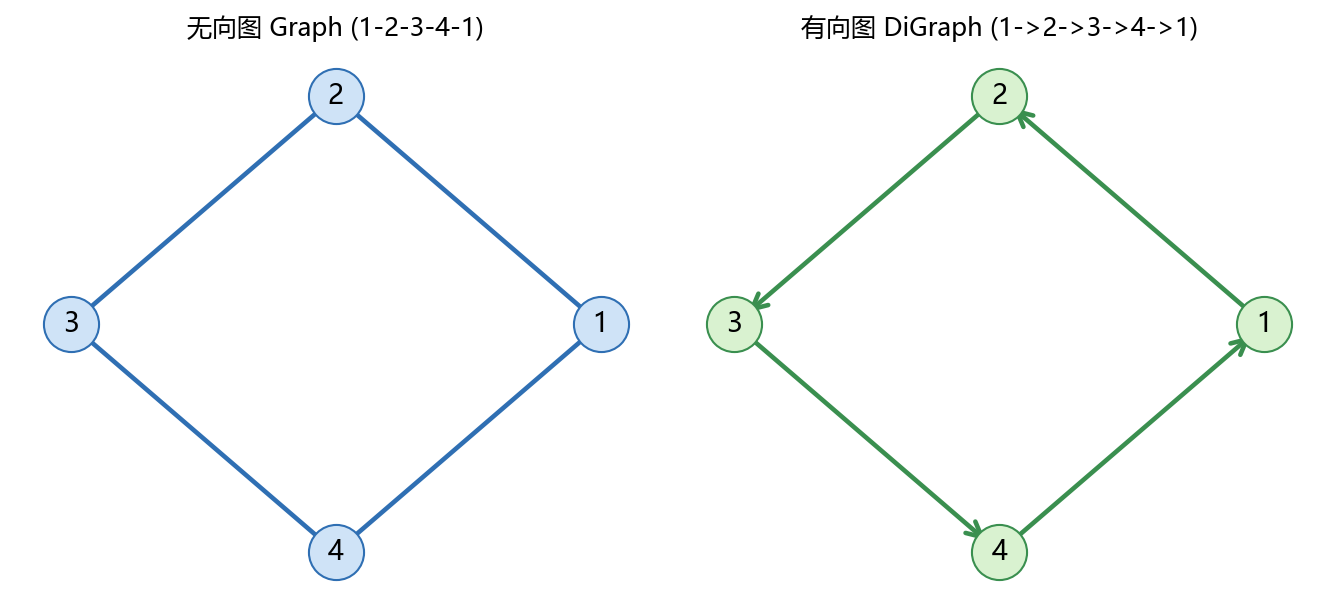
\includegraphics[keepaspectratio,alt={无向图与有向图示例}]{figures/06-networkx/graph_basic.png}}
\caption{无向图与有向图示例}
\end{figure}

\begin{center}\rule{0.5\linewidth}{0.5pt}\end{center}

\subsection{1.3
创建有向图（DiGraph）}\label{ux521bux5efaux6709ux5411ux56fedigraph}

有向图的边有方向，用 nx.DiGraph 创建。

\begin{Shaded}
\begin{Highlighting}[]
\ImportTok{import}\NormalTok{ networkx }\ImportTok{as}\NormalTok{ nx}

\NormalTok{DG }\OperatorTok{=}\NormalTok{ nx.DiGraph()}
\NormalTok{DG.add\_node(}\DecValTok{1}\NormalTok{)}
\NormalTok{DG.add\_nodes\_from([}\DecValTok{2}\NormalTok{, }\DecValTok{3}\NormalTok{, }\DecValTok{4}\NormalTok{])}
\NormalTok{DG.add\_edge(}\DecValTok{1}\NormalTok{, }\DecValTok{2}\NormalTok{)}
\NormalTok{DG.add\_edges\_from([(}\DecValTok{2}\NormalTok{, }\DecValTok{3}\NormalTok{), (}\DecValTok{3}\NormalTok{, }\DecValTok{4}\NormalTok{), (}\DecValTok{4}\NormalTok{, }\DecValTok{1}\NormalTok{)])}

\BuiltInTok{print}\NormalTok{(DG.nodes())}
\BuiltInTok{print}\NormalTok{(DG.edges())}
\end{Highlighting}
\end{Shaded}

\begin{Shaded}
\begin{Highlighting}[]
\NormalTok{[1, 2, 3, 4]}
\NormalTok{[(1, 2), (2, 3), (3, 4), (4, 1)]}
\end{Highlighting}
\end{Shaded}

\subsubsection{1.3.1
入度、出度、前驱与后继}\label{ux5165ux5ea6ux51faux5ea6ux524dux9a71ux4e0eux540eux7ee7}

\begin{Shaded}
\begin{Highlighting}[]
\BuiltInTok{print}\NormalTok{(DG.in\_degree())}
\BuiltInTok{print}\NormalTok{(DG.out\_degree())}
\ControlFlowTok{for}\NormalTok{ node }\KeywordTok{in}\NormalTok{ DG.nodes():}
    \BuiltInTok{print}\NormalTok{(}\StringTok{"Node"}\NormalTok{, node, }\StringTok{"in{-}degree"}\NormalTok{, DG.in\_degree(node), }\StringTok{"out{-}degree"}\NormalTok{, DG.out\_degree(node))}
\BuiltInTok{print}\NormalTok{(}\BuiltInTok{list}\NormalTok{(DG.predecessors(}\DecValTok{2}\NormalTok{)))   }\CommentTok{\# 指向 2 的节点}
\BuiltInTok{print}\NormalTok{(}\BuiltInTok{list}\NormalTok{(DG.successors(}\DecValTok{2}\NormalTok{)))     }\CommentTok{\# 2 指向的节点}
\end{Highlighting}
\end{Shaded}

\begin{Shaded}
\begin{Highlighting}[]
\NormalTok{[(1, 1), (2, 1), (3, 1), (4, 1)]}
\NormalTok{[(1, 1), (2, 1), (3, 1), (4, 1)]}
\NormalTok{Node 1 in{-}degree 1 out{-}degree 1}
\NormalTok{Node 2 in{-}degree 1 out{-}degree 1}
\NormalTok{Node 3 in{-}degree 1 out{-}degree 1}
\NormalTok{Node 4 in{-}degree 1 out{-}degree 1}
\NormalTok{[1]}
\NormalTok{[3]}
\end{Highlighting}
\end{Shaded}

\begin{quote}
注意：原始资料里用 zip(nodes, in\_degree, out\_degree)
的写法会把元组拆错（in\_degree 返回的是 (节点, 度数)
对）。建议像上面这样用 DG.in\_degree(node) 单独取度数，或用
dict(DG.in\_degree())。
\end{quote}

\subsubsection{1.3.2
强连通与弱连通}\label{ux5f3aux8fdeux901aux4e0eux5f31ux8fdeux901a}

有向图的连通性要区分：

\begin{itemize}
\tightlist
\item
  强连通：任意两点都互相可达；
\item
  弱连通：忽略方向后，任意两点可达。
\end{itemize}

\begin{Shaded}
\begin{Highlighting}[]
\BuiltInTok{print}\NormalTok{(nx.is\_strongly\_connected(DG))}
\BuiltInTok{print}\NormalTok{(nx.is\_weakly\_connected(DG))}
\end{Highlighting}
\end{Shaded}

\begin{Shaded}
\begin{Highlighting}[]
\NormalTok{True}
\NormalTok{True}
\end{Highlighting}
\end{Shaded}

\subsubsection{1.3.3 有向图遍历}\label{ux6709ux5411ux56feux904dux5386}

\begin{Shaded}
\begin{Highlighting}[]
\BuiltInTok{print}\NormalTok{(}\BuiltInTok{list}\NormalTok{(nx.dfs\_preorder\_nodes(DG, source}\OperatorTok{=}\DecValTok{1}\NormalTok{)))}
\BuiltInTok{print}\NormalTok{(}\BuiltInTok{list}\NormalTok{(nx.bfs\_edges(DG, source}\OperatorTok{=}\DecValTok{1}\NormalTok{)))}
\end{Highlighting}
\end{Shaded}

\begin{Shaded}
\begin{Highlighting}[]
\NormalTok{[1, 2, 3, 4]}
\NormalTok{[(1, 2), (2, 3), (3, 4)]}
\end{Highlighting}
\end{Shaded}

绘图时 NetworkX 会根据有向性画箭头：

\begin{Shaded}
\begin{Highlighting}[]
\ImportTok{import}\NormalTok{ matplotlib.pyplot }\ImportTok{as}\NormalTok{ plt}
\NormalTok{nx.draw(DG, with\_labels}\OperatorTok{=}\VariableTok{True}\NormalTok{, font\_weight}\OperatorTok{=}\StringTok{"bold"}\NormalTok{, arrowstyle}\OperatorTok{=}\StringTok{"{-}\textgreater{}"}\NormalTok{, arrowsize}\OperatorTok{=}\DecValTok{20}\NormalTok{)}
\NormalTok{plt.show()}
\end{Highlighting}
\end{Shaded}

\begin{center}\rule{0.5\linewidth}{0.5pt}\end{center}

\subsection{1.4
节点与边属性、加权图}\label{ux8282ux70b9ux4e0eux8fb9ux5c5eux6027ux52a0ux6743ux56fe}

\subsubsection{1.4.1 权重（weight）}\label{ux6743ux91cdweight}

\begin{Shaded}
\begin{Highlighting}[]
\NormalTok{G }\OperatorTok{=}\NormalTok{ nx.Graph()}
\NormalTok{G.add\_weighted\_edges\_from([(}\StringTok{"A"}\NormalTok{, }\StringTok{"B"}\NormalTok{, }\DecValTok{10}\NormalTok{), (}\StringTok{"A"}\NormalTok{, }\StringTok{"C"}\NormalTok{, }\DecValTok{6}\NormalTok{), (}\StringTok{"B"}\NormalTok{, }\StringTok{"C"}\NormalTok{, }\DecValTok{5}\NormalTok{)])}
\BuiltInTok{print}\NormalTok{(}\BuiltInTok{list}\NormalTok{(G.edges(data}\OperatorTok{=}\VariableTok{True}\NormalTok{)))}
\BuiltInTok{print}\NormalTok{(G[}\StringTok{"A"}\NormalTok{][}\StringTok{"B"}\NormalTok{])                    }\CommentTok{\# 取出 A{-}B 边的属性字典}
\BuiltInTok{print}\NormalTok{(G.degree())                     }\CommentTok{\# 普通度}
\BuiltInTok{print}\NormalTok{(G.degree(weight}\OperatorTok{=}\StringTok{"weight"}\NormalTok{))      }\CommentTok{\# 加权度（点强度）}
\end{Highlighting}
\end{Shaded}

\begin{Shaded}
\begin{Highlighting}[]
\NormalTok{[(\textquotesingle{}A\textquotesingle{}, \textquotesingle{}B\textquotesingle{}, \{\textquotesingle{}weight\textquotesingle{}: 10\}), (\textquotesingle{}A\textquotesingle{}, \textquotesingle{}C\textquotesingle{}, \{\textquotesingle{}weight\textquotesingle{}: 6\}), (\textquotesingle{}B\textquotesingle{}, \textquotesingle{}C\textquotesingle{}, \{\textquotesingle{}weight\textquotesingle{}: 5\})]}
\NormalTok{\{\textquotesingle{}weight\textquotesingle{}: 10\}}
\NormalTok{[(\textquotesingle{}A\textquotesingle{}, 2), (\textquotesingle{}B\textquotesingle{}, 2), (\textquotesingle{}C\textquotesingle{}, 2)]}
\NormalTok{[(\textquotesingle{}A\textquotesingle{}, 16), (\textquotesingle{}B\textquotesingle{}, 15), (\textquotesingle{}C\textquotesingle{}, 11)]}
\end{Highlighting}
\end{Shaded}

\begin{quote}
点强度（weighted degree）是节点所有相连边的权重和：A 连
B(10)、C(6)，所以是 16。加权网络上``重要节点''的衡量常从点强度出发。
\end{quote}

\subsubsection{1.4.2 节点属性}\label{ux8282ux70b9ux5c5eux6027}

\begin{Shaded}
\begin{Highlighting}[]
\NormalTok{G.add\_node(}\StringTok{"A"}\NormalTok{, role}\OperatorTok{=}\StringTok{"hub"}\NormalTok{, color}\OperatorTok{=}\StringTok{"red"}\NormalTok{)}
\BuiltInTok{print}\NormalTok{(}\BuiltInTok{list}\NormalTok{(G.nodes(data}\OperatorTok{=}\VariableTok{True}\NormalTok{)))}
\end{Highlighting}
\end{Shaded}

\begin{Shaded}
\begin{Highlighting}[]
\NormalTok{[(\textquotesingle{}A\textquotesingle{}, \{\textquotesingle{}role\textquotesingle{}: \textquotesingle{}hub\textquotesingle{}, \textquotesingle{}color\textquotesingle{}: \textquotesingle{}red\textquotesingle{}\}), (\textquotesingle{}B\textquotesingle{}, \{\}), (\textquotesingle{}C\textquotesingle{}, \{\})]}
\end{Highlighting}
\end{Shaded}

节点/边上可以挂任意字典属性；用 G.nodes(data=True) 与 G.edges(data=True)
一起查看。

\begin{center}\rule{0.5\linewidth}{0.5pt}\end{center}

\subsection{1.5
常用图生成器}\label{ux5e38ux7528ux56feux751fux6210ux5668}

NetworkX 自带许多``造图''模板，适合课堂演示与随机网络实验。

\begin{Shaded}
\begin{Highlighting}[]
\BuiltInTok{print}\NormalTok{(}\BuiltInTok{list}\NormalTok{(nx.path\_graph(}\DecValTok{6}\NormalTok{).edges()))}
\BuiltInTok{print}\NormalTok{(}\BuiltInTok{list}\NormalTok{(nx.cycle\_graph(}\DecValTok{5}\NormalTok{).edges()))}
\BuiltInTok{print}\NormalTok{(}\BuiltInTok{list}\NormalTok{(nx.complete\_graph(}\DecValTok{4}\NormalTok{).edges()))}
\BuiltInTok{print}\NormalTok{(}\BuiltInTok{list}\NormalTok{(nx.star\_graph(}\DecValTok{5}\NormalTok{).edges()))}
\BuiltInTok{print}\NormalTok{(}\BuiltInTok{list}\NormalTok{(nx.grid\_2d\_graph(}\DecValTok{2}\NormalTok{, }\DecValTok{3}\NormalTok{).nodes()))}
\BuiltInTok{print}\NormalTok{(}\BuiltInTok{list}\NormalTok{(nx.grid\_2d\_graph(}\DecValTok{2}\NormalTok{, }\DecValTok{3}\NormalTok{).edges()))}
\NormalTok{K }\OperatorTok{=}\NormalTok{ nx.karate\_club\_graph()}
\BuiltInTok{print}\NormalTok{(}\StringTok{"karate\_club:"}\NormalTok{, K.number\_of\_nodes(), K.number\_of\_edges())}
\end{Highlighting}
\end{Shaded}

\begin{Shaded}
\begin{Highlighting}[]
\NormalTok{[(0, 1), (1, 2), (2, 3), (3, 4), (4, 5)]}
\NormalTok{[(0, 1), (0, 4), (1, 2), (2, 3), (3, 4)]}
\NormalTok{[(0, 1), (0, 2), (0, 3), (1, 2), (1, 3), (2, 3)]}
\NormalTok{[(0, 1), (0, 2), (0, 3), (0, 4), (0, 5)]}
\NormalTok{[(0, 0), (0, 1), (0, 2), (1, 0), (1, 1), (1, 2)]}
\NormalTok{[((0, 0), (1, 0)), ((0, 0), (0, 1)), ((0, 1), (1, 1)), ((0, 1), (0, 2)), ((0, 2), (1, 2)), ((1, 0), (1, 1)), ((1, 1), (1, 2))]}
\NormalTok{karate\_club: 34 78}
\end{Highlighting}
\end{Shaded}

随机网络生成器通常带 seed 参数，保证结果可复现：

\begin{Shaded}
\begin{Highlighting}[]
\NormalTok{er }\OperatorTok{=}\NormalTok{ nx.erdos\_renyi\_graph(}\DecValTok{10}\NormalTok{, }\FloatTok{0.3}\NormalTok{, seed}\OperatorTok{=}\DecValTok{42}\NormalTok{)}
\NormalTok{ws }\OperatorTok{=}\NormalTok{ nx.watts\_strogatz\_graph(}\DecValTok{10}\NormalTok{, }\DecValTok{4}\NormalTok{, }\FloatTok{0.1}\NormalTok{, seed}\OperatorTok{=}\DecValTok{42}\NormalTok{)}
\NormalTok{ba }\OperatorTok{=}\NormalTok{ nx.barabasi\_albert\_graph(}\DecValTok{10}\NormalTok{, }\DecValTok{2}\NormalTok{, seed}\OperatorTok{=}\DecValTok{42}\NormalTok{)}
\BuiltInTok{print}\NormalTok{(}\StringTok{"erdos\_renyi:"}\NormalTok{, er.number\_of\_nodes(), er.number\_of\_edges())}
\BuiltInTok{print}\NormalTok{(}\StringTok{"watts\_strogatz:"}\NormalTok{, ws.number\_of\_nodes(), ws.number\_of\_edges())}
\BuiltInTok{print}\NormalTok{(}\StringTok{"barabasi\_albert:"}\NormalTok{, ba.number\_of\_nodes(), ba.number\_of\_edges())}
\end{Highlighting}
\end{Shaded}

\begin{Shaded}
\begin{Highlighting}[]
\NormalTok{erdos\_renyi: 10 17}
\NormalTok{watts\_strogatz: 10 20}
\NormalTok{barabasi\_albert: 10 16}
\end{Highlighting}
\end{Shaded}

\begin{center}\rule{0.5\linewidth}{0.5pt}\end{center}

\subsection{1.6 邻接矩阵（与 NumPy
对接）}\label{ux90bbux63a5ux77e9ux9635ux4e0e-numpy-ux5bf9ux63a5}

用 nx.to\_numpy\_array 可把图转成邻接矩阵，便于交给 NumPy/SciPy
做数值计算。

\begin{Shaded}
\begin{Highlighting}[]
\ImportTok{import}\NormalTok{ numpy }\ImportTok{as}\NormalTok{ np}
\NormalTok{G }\OperatorTok{=}\NormalTok{ nx.Graph()}
\NormalTok{G.add\_edges\_from([(}\DecValTok{1}\NormalTok{, }\DecValTok{2}\NormalTok{), (}\DecValTok{2}\NormalTok{, }\DecValTok{3}\NormalTok{), (}\DecValTok{3}\NormalTok{, }\DecValTok{1}\NormalTok{), (}\DecValTok{3}\NormalTok{, }\DecValTok{4}\NormalTok{)])}
\NormalTok{A }\OperatorTok{=}\NormalTok{ nx.to\_numpy\_array(G)}
\BuiltInTok{print}\NormalTok{(A)}
\end{Highlighting}
\end{Shaded}

\begin{Shaded}
\begin{Highlighting}[]
\NormalTok{[[0. 1. 1. 0.]}
\NormalTok{ [1. 0. 1. 0.]}
\NormalTok{ [1. 1. 0. 1.]}
\NormalTok{ [0. 0. 1. 0.]]}
\end{Highlighting}
\end{Shaded}

有向图会得到非对称矩阵：

\begin{Shaded}
\begin{Highlighting}[]
\NormalTok{D }\OperatorTok{=}\NormalTok{ nx.DiGraph()}\OperatorTok{;}\NormalTok{ D.add\_edges\_from([(}\DecValTok{1}\NormalTok{, }\DecValTok{2}\NormalTok{), (}\DecValTok{2}\NormalTok{, }\DecValTok{3}\NormalTok{), (}\DecValTok{3}\NormalTok{, }\DecValTok{1}\NormalTok{), (}\DecValTok{2}\NormalTok{, }\DecValTok{4}\NormalTok{)])}
\BuiltInTok{print}\NormalTok{(nx.to\_numpy\_array(D))}
\end{Highlighting}
\end{Shaded}

\begin{Shaded}
\begin{Highlighting}[]
\NormalTok{[[0. 1. 0. 0.]}
\NormalTok{ [0. 0. 1. 1.]}
\NormalTok{ [1. 0. 0. 0.]}
\NormalTok{ [0. 0. 0. 0.]]}
\end{Highlighting}
\end{Shaded}

\subsection{案例卡 1：用 nx.Graph
建``班级社交网''------节点/边/属性/度}\label{ux6848ux4f8bux5361-1ux7528-nx.graph-ux5efaux73edux7ea7ux793eux4ea4ux7f51ux8282ux70b9ux8fb9ux5c5eux6027ux5ea6}

\subsubsection{目标}\label{ux76eeux6807-24}

把 5 位同学当成``节点''，把``一起学习/讨论''当成``边''，用
\texttt{nx.Graph}
建一张班级社交网。你会顺带掌握：给节点挂属性、给边加权重（每周讨论次数）、看每个节点的\textbf{度}（直接朋友数）与\textbf{点强度}（加权度=朋友往来总次数）。

\subsubsection{代码}\label{ux4ee3ux7801-25}

\begin{Shaded}
\begin{Highlighting}[]
\ImportTok{import}\NormalTok{ networkx }\ImportTok{as}\NormalTok{ nx}
\ImportTok{import}\NormalTok{ matplotlib.pyplot }\ImportTok{as}\NormalTok{ plt}
\ImportTok{import}\NormalTok{ numpy }\ImportTok{as}\NormalTok{ np}
\ImportTok{import}\NormalTok{ os}

\NormalTok{plt.rcParams[}\StringTok{\textquotesingle{}font.sans{-}serif\textquotesingle{}}\NormalTok{] }\OperatorTok{=}\NormalTok{ [}\StringTok{\textquotesingle{}Microsoft YaHei\textquotesingle{}}\NormalTok{, }\StringTok{\textquotesingle{}SimHei\textquotesingle{}}\NormalTok{, }\StringTok{\textquotesingle{}DejaVu Sans\textquotesingle{}}\NormalTok{]}
\NormalTok{plt.rcParams[}\StringTok{\textquotesingle{}axes.unicode\_minus\textquotesingle{}}\NormalTok{] }\OperatorTok{=} \VariableTok{False}
\NormalTok{np.set\_printoptions(precision}\OperatorTok{=}\DecValTok{4}\NormalTok{, suppress}\OperatorTok{=}\VariableTok{True}\NormalTok{)}

\CommentTok{\#\# 1) 建空图}
\NormalTok{G }\OperatorTok{=}\NormalTok{ nx.Graph()}

\CommentTok{\#\# 2) 一次加多个节点，并给每个节点挂属性(班级/兴趣)}
\NormalTok{students }\OperatorTok{=}\NormalTok{ [}
\NormalTok{    (}\StringTok{\textquotesingle{}小明\textquotesingle{}}\NormalTok{, \{}\StringTok{\textquotesingle{}cls\textquotesingle{}}\NormalTok{: }\StringTok{\textquotesingle{}一班\textquotesingle{}}\NormalTok{, }\StringTok{\textquotesingle{}interest\textquotesingle{}}\NormalTok{: }\StringTok{\textquotesingle{}数学\textquotesingle{}}\NormalTok{\}),}
\NormalTok{    (}\StringTok{\textquotesingle{}小红\textquotesingle{}}\NormalTok{, \{}\StringTok{\textquotesingle{}cls\textquotesingle{}}\NormalTok{: }\StringTok{\textquotesingle{}一班\textquotesingle{}}\NormalTok{, }\StringTok{\textquotesingle{}interest\textquotesingle{}}\NormalTok{: }\StringTok{\textquotesingle{}编程\textquotesingle{}}\NormalTok{\}),}
\NormalTok{    (}\StringTok{\textquotesingle{}小刚\textquotesingle{}}\NormalTok{, \{}\StringTok{\textquotesingle{}cls\textquotesingle{}}\NormalTok{: }\StringTok{\textquotesingle{}一班\textquotesingle{}}\NormalTok{, }\StringTok{\textquotesingle{}interest\textquotesingle{}}\NormalTok{: }\StringTok{\textquotesingle{}物理\textquotesingle{}}\NormalTok{\}),}
\NormalTok{    (}\StringTok{\textquotesingle{}小丽\textquotesingle{}}\NormalTok{, \{}\StringTok{\textquotesingle{}cls\textquotesingle{}}\NormalTok{: }\StringTok{\textquotesingle{}二班\textquotesingle{}}\NormalTok{, }\StringTok{\textquotesingle{}interest\textquotesingle{}}\NormalTok{: }\StringTok{\textquotesingle{}语文\textquotesingle{}}\NormalTok{\}),}
\NormalTok{    (}\StringTok{\textquotesingle{}小华\textquotesingle{}}\NormalTok{, \{}\StringTok{\textquotesingle{}cls\textquotesingle{}}\NormalTok{: }\StringTok{\textquotesingle{}二班\textquotesingle{}}\NormalTok{, }\StringTok{\textquotesingle{}interest\textquotesingle{}}\NormalTok{: }\StringTok{\textquotesingle{}美术\textquotesingle{}}\NormalTok{\}),}
\NormalTok{]}
\NormalTok{G.add\_nodes\_from(students)}

\CommentTok{\#\# 3) 加边，weight 表示每周一起讨论的次数}
\NormalTok{G.add\_weighted\_edges\_from([}
\NormalTok{    (}\StringTok{\textquotesingle{}小明\textquotesingle{}}\NormalTok{, }\StringTok{\textquotesingle{}小红\textquotesingle{}}\NormalTok{, }\DecValTok{3}\NormalTok{),}
\NormalTok{    (}\StringTok{\textquotesingle{}小明\textquotesingle{}}\NormalTok{, }\StringTok{\textquotesingle{}小刚\textquotesingle{}}\NormalTok{, }\DecValTok{2}\NormalTok{),}
\NormalTok{    (}\StringTok{\textquotesingle{}小红\textquotesingle{}}\NormalTok{, }\StringTok{\textquotesingle{}小刚\textquotesingle{}}\NormalTok{, }\DecValTok{4}\NormalTok{),}
\NormalTok{    (}\StringTok{\textquotesingle{}小刚\textquotesingle{}}\NormalTok{, }\StringTok{\textquotesingle{}小丽\textquotesingle{}}\NormalTok{, }\DecValTok{1}\NormalTok{),}
\NormalTok{    (}\StringTok{\textquotesingle{}小丽\textquotesingle{}}\NormalTok{, }\StringTok{\textquotesingle{}小华\textquotesingle{}}\NormalTok{, }\DecValTok{5}\NormalTok{),}
\NormalTok{])}

\BuiltInTok{print}\NormalTok{(}\StringTok{\textquotesingle{}节点数:\textquotesingle{}}\NormalTok{, G.number\_of\_nodes(), }\StringTok{\textquotesingle{}  边数:\textquotesingle{}}\NormalTok{, G.number\_of\_edges())}
\BuiltInTok{print}\NormalTok{(}\StringTok{\textquotesingle{}节点及属性:\textquotesingle{}}\NormalTok{)}
\ControlFlowTok{for}\NormalTok{ n, data }\KeywordTok{in}\NormalTok{ G.nodes(data}\OperatorTok{=}\VariableTok{True}\NormalTok{):}
    \BuiltInTok{print}\NormalTok{(}\StringTok{\textquotesingle{} \textquotesingle{}}\NormalTok{, n, data)}
\BuiltInTok{print}\NormalTok{(}\StringTok{\textquotesingle{}边及权重:\textquotesingle{}}\NormalTok{)}
\ControlFlowTok{for}\NormalTok{ u, v, w }\KeywordTok{in}\NormalTok{ G.edges(data}\OperatorTok{=}\StringTok{\textquotesingle{}weight\textquotesingle{}}\NormalTok{):}
    \BuiltInTok{print}\NormalTok{(}\SpecialStringTok{f\textquotesingle{}  }\SpecialCharTok{\{}\NormalTok{u}\SpecialCharTok{\}}\SpecialStringTok{ {-}{-} }\SpecialCharTok{\{}\NormalTok{v}\SpecialCharTok{\}}\SpecialStringTok{ : }\SpecialCharTok{\{}\NormalTok{w}\SpecialCharTok{\}}\SpecialStringTok{\textquotesingle{}}\NormalTok{)}

\CommentTok{\#\# 4) 度 与 点强度(加权度)}
\BuiltInTok{print}\NormalTok{(}\StringTok{\textquotesingle{}每个节点的度(降序):\textquotesingle{}}\NormalTok{, }\BuiltInTok{sorted}\NormalTok{(}\BuiltInTok{dict}\NormalTok{(G.degree()).items(), key}\OperatorTok{=}\KeywordTok{lambda}\NormalTok{ x: (}\OperatorTok{{-}}\NormalTok{x[}\DecValTok{1}\NormalTok{], x[}\DecValTok{0}\NormalTok{])))}
\BuiltInTok{print}\NormalTok{(}\StringTok{\textquotesingle{}每个节点的加权度/点强度(降序):\textquotesingle{}}\NormalTok{,}
      \BuiltInTok{sorted}\NormalTok{(}\BuiltInTok{dict}\NormalTok{(G.degree(weight}\OperatorTok{=}\StringTok{\textquotesingle{}weight\textquotesingle{}}\NormalTok{)).items(), key}\OperatorTok{=}\KeywordTok{lambda}\NormalTok{ x: (}\OperatorTok{{-}}\NormalTok{x[}\DecValTok{1}\NormalTok{], x[}\DecValTok{0}\NormalTok{])))}

\CommentTok{\#\# 5) 画出来(jupyter 里可直接显示；脚本环境保存到 figures/06{-}networkx/)}
\NormalTok{os.makedirs(}\StringTok{\textquotesingle{}images\textquotesingle{}}\NormalTok{, exist\_ok}\OperatorTok{=}\VariableTok{True}\NormalTok{)}
\NormalTok{pos }\OperatorTok{=}\NormalTok{ nx.spring\_layout(G, seed}\OperatorTok{=}\DecValTok{42}\NormalTok{, k}\OperatorTok{=}\FloatTok{0.8}\NormalTok{)}
\NormalTok{plt.figure(figsize}\OperatorTok{=}\NormalTok{(}\FloatTok{6.4}\NormalTok{, }\FloatTok{4.6}\NormalTok{))}
\NormalTok{nx.draw\_networkx\_nodes(G, pos, node\_size}\OperatorTok{=}\DecValTok{800}\NormalTok{, node\_color}\OperatorTok{=}\StringTok{\textquotesingle{}\#cfe3f7\textquotesingle{}}\NormalTok{, edgecolors}\OperatorTok{=}\StringTok{\textquotesingle{}\#2f6fb3\textquotesingle{}}\NormalTok{)}
\NormalTok{nx.draw\_networkx\_edges(G, pos, width}\OperatorTok{=}\FloatTok{2.0}\NormalTok{, edge\_color}\OperatorTok{=}\StringTok{\textquotesingle{}\#4b8bbe\textquotesingle{}}\NormalTok{)}
\NormalTok{nx.draw\_networkx\_labels(G, pos, font\_size}\OperatorTok{=}\DecValTok{11}\NormalTok{, font\_family}\OperatorTok{=}\StringTok{\textquotesingle{}Microsoft YaHei\textquotesingle{}}\NormalTok{)}
\NormalTok{plt.title(}\StringTok{\textquotesingle{}班级社交网\textquotesingle{}}\NormalTok{)}
\NormalTok{plt.axis(}\StringTok{\textquotesingle{}off\textquotesingle{}}\NormalTok{)}
\NormalTok{plt.tight\_layout()}
\NormalTok{plt.savefig(}\StringTok{\textquotesingle{}figures/06{-}networkx/case1\_class\_network.png\textquotesingle{}}\NormalTok{, dpi}\OperatorTok{=}\DecValTok{150}\NormalTok{)}
\BuiltInTok{print}\NormalTok{(}\StringTok{\textquotesingle{}已保存 figures/06{-}networkx/case1\_class\_network.png\textquotesingle{}}\NormalTok{)}
\NormalTok{plt.close()}
\end{Highlighting}
\end{Shaded}

\subsubsection{运行结果(已运行核验)}\label{ux8fd0ux884cux7ed3ux679cux5df2ux8fd0ux884cux6838ux9a8c-23}

\begin{Shaded}
\begin{Highlighting}[]
\NormalTok{节点数: 5   边数: 5}
\NormalTok{节点及属性:}
\NormalTok{  小明 \{\textquotesingle{}cls\textquotesingle{}: \textquotesingle{}一班\textquotesingle{}, \textquotesingle{}interest\textquotesingle{}: \textquotesingle{}数学\textquotesingle{}\}}
\NormalTok{  小红 \{\textquotesingle{}cls\textquotesingle{}: \textquotesingle{}一班\textquotesingle{}, \textquotesingle{}interest\textquotesingle{}: \textquotesingle{}编程\textquotesingle{}\}}
\NormalTok{  小刚 \{\textquotesingle{}cls\textquotesingle{}: \textquotesingle{}一班\textquotesingle{}, \textquotesingle{}interest\textquotesingle{}: \textquotesingle{}物理\textquotesingle{}\}}
\NormalTok{  小丽 \{\textquotesingle{}cls\textquotesingle{}: \textquotesingle{}二班\textquotesingle{}, \textquotesingle{}interest\textquotesingle{}: \textquotesingle{}语文\textquotesingle{}\}}
\NormalTok{  小华 \{\textquotesingle{}cls\textquotesingle{}: \textquotesingle{}二班\textquotesingle{}, \textquotesingle{}interest\textquotesingle{}: \textquotesingle{}美术\textquotesingle{}\}}
\NormalTok{边及权重:}
\NormalTok{  小明 {-}{-} 小红 : 3}
\NormalTok{  小明 {-}{-} 小刚 : 2}
\NormalTok{  小红 {-}{-} 小刚 : 4}
\NormalTok{  小刚 {-}{-} 小丽 : 1}
\NormalTok{  小丽 {-}{-} 小华 : 5}
\NormalTok{每个节点的度(降序): [(\textquotesingle{}小刚\textquotesingle{}, 3), (\textquotesingle{}小丽\textquotesingle{}, 2), (\textquotesingle{}小明\textquotesingle{}, 2), (\textquotesingle{}小红\textquotesingle{}, 2), (\textquotesingle{}小华\textquotesingle{}, 1)]}
\NormalTok{每个节点的加权度/点强度(降序): [(\textquotesingle{}小刚\textquotesingle{}, 7), (\textquotesingle{}小红\textquotesingle{}, 7), (\textquotesingle{}小丽\textquotesingle{}, 6), (\textquotesingle{}小华\textquotesingle{}, 5), (\textquotesingle{}小明\textquotesingle{}, 5)]}
\NormalTok{已保存 figures/06{-}networkx/case1\_class\_network.png}
\end{Highlighting}
\end{Shaded}

\subsubsection{讲解}\label{ux8bb2ux89e3-23}

\textbf{一句话解释}：先画一张``人=点、一起学习=连线''的网；每条线还能记一个数（每周讨论几次），这样不但知道``谁朋友多''，还知道``谁和朋友来往最勤''。

\begin{enumerate}
\def\labelenumi{\arabic{enumi}.}
\tightlist
\item
  \texttt{G\ =\ nx.Graph()} 建一张\textbf{无向图}：朋友关系不分方向，A
  和 B 是朋友就等于 B 和 A 是朋友。
\item
  \texttt{G.add\_nodes\_from(students)} 里每个元素是
  \texttt{(节点名,\ 属性字典)}，所以一次就能把``班级、兴趣''挂在节点上；查看时用
  \texttt{G.nodes(data=True)} 会得到 \texttt{(节点,\ 属性字典)} 对。
\item
  \texttt{G.add\_weighted\_edges\_from(...)} 的每个元素是
  \texttt{(起点,\ 终点,\ 权重)}；\texttt{weight} 是 NetworkX
  约定好的边属性名，后面
  \texttt{degree(weight=\textquotesingle{}weight\textquotesingle{})}
  才能自动读到它。
\item
  \texttt{G.degree()} 是\textbf{直接邻居数}：小明连小红、小刚，所以是
  2；小刚连小明、小红、小丽，是 3。
\item
  \texttt{G.degree(weight=\textquotesingle{}weight\textquotesingle{})}
  是把``每条边的权重相加''，等于\textbf{点强度}：小刚=2+4+1=7，小红=3+4=7，小丽=1+5=6，小华=5，小明=3+2=5。所以小刚虽然度最高，但``来往总次数''第一的是小刚和小红并列。
\item
  \texttt{nx.spring\_layout(G,\ seed=42)} 给节点随机选初始位置，固定
  \texttt{seed=42} 才能每次画出同一张布局；保存到
  \texttt{figures/06-networkx/} 前先
  \texttt{os.makedirs(\textquotesingle{}images\textquotesingle{},\ exist\_ok=True)}，避免目录不存在报错。
\end{enumerate}

\begin{figure}
\centering
\pandocbounded{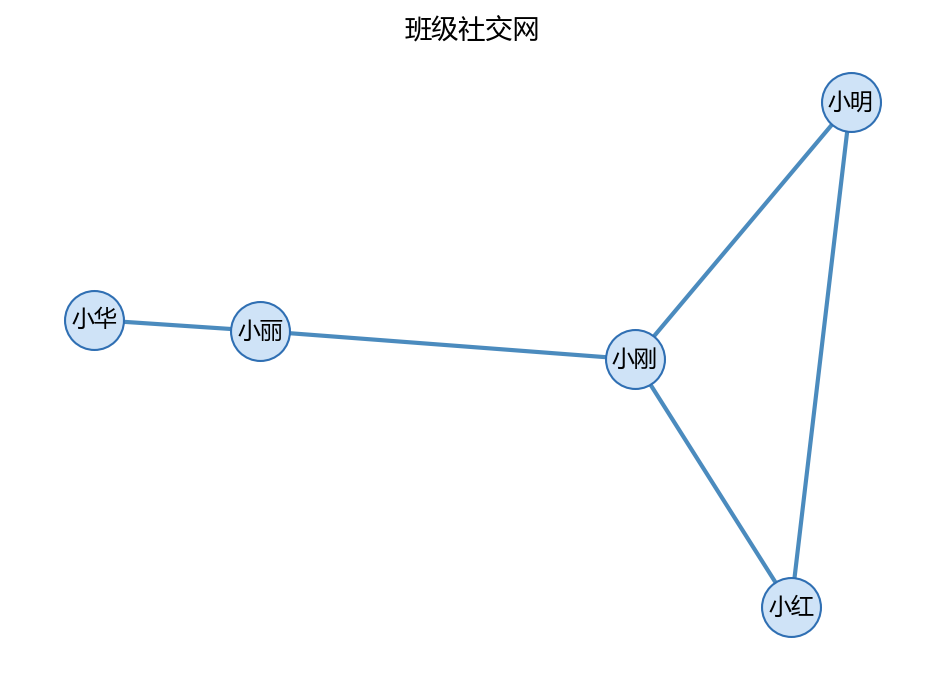
\includegraphics[keepaspectratio,alt={班级社交网}]{figures/06-networkx/case1_class_network.png}}
\caption{班级社交网}
\end{figure}

\subsubsection{主要用法 / API}\label{ux4e3bux8981ux7528ux6cd5-api-24}

{\def\LTcaptype{none} % do not increment counter
\begin{longtable}[]{@{}
  >{\raggedright\arraybackslash}p{(\linewidth - 4\tabcolsep) * \real{0.3333}}
  >{\raggedright\arraybackslash}p{(\linewidth - 4\tabcolsep) * \real{0.3333}}
  >{\raggedright\arraybackslash}p{(\linewidth - 4\tabcolsep) * \real{0.3333}}@{}}
\toprule\noalign{}
\begin{minipage}[b]{\linewidth}\raggedright
需求
\end{minipage} & \begin{minipage}[b]{\linewidth}\raggedright
写法
\end{minipage} & \begin{minipage}[b]{\linewidth}\raggedright
说明
\end{minipage} \\
\midrule\noalign{}
\endhead
\bottomrule\noalign{}
\endlastfoot
建空无向图 & \texttt{nx.Graph()} & 边无方向 \\
加单个/多个节点 & \texttt{add\_node} / \texttt{add\_nodes\_from} &
可带属性 \\
加单条/多条边 & \texttt{add\_edge} / \texttt{add\_edges\_from} &
无向图自动补反向 \\
加带权边 & \texttt{add\_weighted\_edges\_from({[}(u,\ v,\ w){]})} &
属性名 \texttt{weight} \\
查看节点/边属性 & \texttt{G.nodes(data=True)} /
\texttt{G.edges(data=True)} & 得到 \texttt{(节点,\ dict)} /
\texttt{(u,\ v,\ dict)} \\
度 & \texttt{G.degree()} / \texttt{G.degree(node)} & 直接邻居数 \\
点强度 &
\texttt{G.degree(weight=\textquotesingle{}weight\textquotesingle{})} &
加权度 \\
画图 & \texttt{nx.draw\_networkx\_*} + \texttt{plt.savefig} &
需配中文字体 \\
\end{longtable}
}

\subsubsection{常见错误}\label{ux5e38ux89c1ux9519ux8bef-24}

\begin{enumerate}
\def\labelenumi{\arabic{enumi}.}
\tightlist
\item
  以为 \texttt{add\_edge(u,\ v,\ 10)} 的第三个参数是权重 → 错误；正解是
  \texttt{add\_edge(u,\ v,\ weight=10)} 或
  \texttt{add\_weighted\_edges\_from}。
\item
  忘记
  \texttt{G.degree(weight=\textquotesingle{}weight\textquotesingle{})}
  的 \texttt{weight} 参数名要跟边属性名一致；如果边属性叫
  \texttt{time}，就要写
  \texttt{weight=\textquotesingle{}time\textquotesingle{}}。
\item
  用 \texttt{plt.show()} 在无界面环境会卡住/无反应 → 脚本/作业里用
  \texttt{plt.savefig(...)}；\texttt{spring\_layout} 不传 \texttt{seed}
  每次布局都不同，作业截图容易对不上。
\item
  \texttt{sorted(G.degree())} 返回的是按节点名排列的
  \texttt{(节点,\ 度)} 列表；想按度数排序要
  \texttt{key=lambda\ x:\ (-x{[}1{]},\ x{[}0{]})}。
\end{enumerate}

\subsubsection{拓展 / 跟练}\label{ux62d3ux5c55-ux8ddfux7ec3-12}

\begin{enumerate}
\def\labelenumi{\arabic{enumi}.}
\tightlist
\item
  新加一位同学 \texttt{小强} 与 \texttt{小华} 连一条权重 2
  的边，再打印度与点强度，看谁变成``朋友最多''。
\item
  把每条边的权重改成``共同爱好数''，分别打印度与点强度，观察两者排名是否一致。
\item
  用
  \texttt{nx.to\_numpy\_array(G,\ nodelist=sorted(G.nodes()),\ weight=\textquotesingle{}weight\textquotesingle{})}
  得到邻接矩阵，验证它是对称矩阵。
\item
  给每个节点补一个 \texttt{age}
  属性，然后筛选出``一班''的学生（答案：\texttt{{[}n\ for\ n,\ d\ in\ G.nodes(data=True)\ if\ d.get(\textquotesingle{}cls\textquotesingle{})==\textquotesingle{}一班\textquotesingle{}{]}}）。
\end{enumerate}

\begin{center}\rule{0.5\linewidth}{0.5pt}\end{center}

\subsection{常见误区}\label{ux5e38ux89c1ux8befux533a-17}

\begin{enumerate}
\def\labelenumi{\arabic{enumi}.}
\tightlist
\item
  \textbf{把 nodes/edges 当普通列表}：它们是视图对象，直接判断成员/转
  list 均可，但不要对它做破坏性修改（例如 G.nodes() 不能赋值）。
\item
  \textbf{在有向图上误用 neighbors}：有向图有前驱与后继两个方向，要用
  predecessors / successors，neighbors 在有向图中返回后继节点。
\item
  \textbf{误用 zip(nodes, in\_degree, out\_degree)}：in\_degree 返回的是
  (节点, 度数) 对，直接解包会把元组整体当成``度数''。建议用
  DG.in\_degree(node) 或 dict(DG.in\_degree())。
\item
  \textbf{忘记给加权边指定 weight 关键字}：add\_weighted\_edges\_from
  默认用 weight 作为属性名；若用 add\_edge 加权重需写成 add\_edge(u, v,
  weight=w)。
\item
  \textbf{随机图不设 seed}：结果每次不同，课堂/作业演示请设 seed（如
  seed=42）。
\item
  \textbf{把图当作``可哈希容器''直接比较}：两个结构相同的图不一定相等，判断是否同构要用
  nx.is\_isomorphic。
\end{enumerate}

\subsection{思考题}\label{ux601dux8003ux9898-19}

\begin{enumerate}
\def\labelenumi{\arabic{enumi}.}
\tightlist
\item
  无向图 G.nodes()
  返回的节点顺序是添加顺序还是自动排序？用循环访问时是否稳定？
\item
  为什么强连通要求``互相可达''？给出一个弱连通但不强连通的有向图例子。
\item
  nx.Graph(G) 与 nx.DiGraph(G) 把一个无向图转成有向图时，边会变成几条？
\end{enumerate}

\subsection{动手练习（详见
lab）}\label{ux52a8ux624bux7ec3ux4e60ux8be6ux89c1-lab-11}

\begin{itemize}
\tightlist
\item
  创建一个 6 节点的无向环图（cycle\_graph），打印每条边与每个节点的度；
\item
  创建一个包含 5 个节点的星形图（star\_graph），找出中心节点并计算其度；
\item
  给一个加权图添加节点属性，打印 nodes(data=True) 与 edges(data=True)；
\item
  用 karate\_club\_graph 生成图并转为邻接矩阵，验证矩阵是 34x34 且对称。
\end{itemize}

\subsection{延伸阅读}\label{ux5ef6ux4f38ux9605ux8bfb-26}

\begin{itemize}
\tightlist
\item
  NetworkX
  官方教程（图基础）：\href{https://networkx.org/documentation/stable/tutorial.html}{链接}
\item
  NetworkX
  官方图类型参考：\href{https://networkx.org/documentation/stable/reference/classes/index.html}{链接}
\item
  NetworkX
  官方生成器列表：\href{https://networkx.org/documentation/stable/reference/generators.html}{链接}
\end{itemize}

\section{02
分析图：结构指标}\label{ux5206ux6790ux56feux7ed3ux6784ux6307ux6807}

\begin{quote}
本节对应原版 6.2 的内容。先给指标下定义，再用 NetworkX
计算，并给出真实运行结果。
\end{quote}

\subsection{本节目标}\label{ux672cux8282ux76eeux6807-24}

\begin{itemize}
\tightlist
\item
  理解度、度分布、平均路径长度、聚类系数、传递性、介数中心性、接近中心性、模块度等指标的含义；
\item
  会用 NetworkX 计算这些指标并读懂结果的数值含义；
\item
  能判断无向图是否连通，有向图是否强连通/弱连通，并提取连通分量；
\item
  会计算加权图的点强度。
\end{itemize}

\subsection{先修}\label{ux5148ux4fee-17}

\begin{itemize}
\tightlist
\item
  第 01 节：创建 Graph / DiGraph，访问 nodes / edges / degree。
\end{itemize}

\begin{center}\rule{0.5\linewidth}{0.5pt}\end{center}

\subsection{2.1 指标一览}\label{ux6307ux6807ux4e00ux89c8}

{\def\LTcaptype{none} % do not increment counter
\begin{longtable}[]{@{}
  >{\raggedright\arraybackslash}p{(\linewidth - 6\tabcolsep) * \real{0.2500}}
  >{\raggedright\arraybackslash}p{(\linewidth - 6\tabcolsep) * \real{0.2500}}
  >{\raggedright\arraybackslash}p{(\linewidth - 6\tabcolsep) * \real{0.2500}}
  >{\raggedright\arraybackslash}p{(\linewidth - 6\tabcolsep) * \real{0.2500}}@{}}
\toprule\noalign{}
\begin{minipage}[b]{\linewidth}\raggedright
指标
\end{minipage} & \begin{minipage}[b]{\linewidth}\raggedright
名字
\end{minipage} & \begin{minipage}[b]{\linewidth}\raggedright
直观含义
\end{minipage} & \begin{minipage}[b]{\linewidth}\raggedright
反映什么
\end{minipage} \\
\midrule\noalign{}
\endhead
\bottomrule\noalign{}
\endlastfoot
度 & Degree & 与节点直接相连的边数 & 节点的``直接影响力'' \\
度分布 & Degree Distribution & 不同度数的节点占比 &
网络拓扑类型（均匀/无标度） \\
平均路径长度 & Average Path Length & 任意两点最短路径边数的均值 &
网络的整体``紧密度/传播效率'' \\
聚类系数 & Clustering Coefficient & 一个节点的邻居彼此相连的程度 &
局部集聚、三角关系 \\
传递性 & Transitivity & 全网三角形与``开放三元组''的比值 &
全局成团倾向 \\
介数中心性 & Betweenness Centrality & 经过该点的最短路径占比 &
节点作为``桥梁/瓶颈''的重要性 \\
接近中心性 & Closeness Centrality & 到其他节点的平均距离越短越接近 &
节点的``可达性/中心程度'' \\
模块度 & Modularity & 社区划分质量 & 网络是否存在明显社区结构 \\
点强度 & Node Strength & 加权度：相连边权重之和 &
加权网络中的``重要性'' \\
\end{longtable}
}

\begin{center}\rule{0.5\linewidth}{0.5pt}\end{center}

\subsection{2.2
节点度与度分布}\label{ux8282ux70b9ux5ea6ux4e0eux5ea6ux5206ux5e03}

\subsubsection{2.2.1 度}\label{ux5ea6}

\begin{Shaded}
\begin{Highlighting}[]
\ImportTok{import}\NormalTok{ networkx }\ImportTok{as}\NormalTok{ nx}

\NormalTok{G }\OperatorTok{=}\NormalTok{ nx.Graph()}
\NormalTok{G.add\_edges\_from([(}\DecValTok{1}\NormalTok{, }\DecValTok{2}\NormalTok{), (}\DecValTok{1}\NormalTok{, }\DecValTok{3}\NormalTok{), (}\DecValTok{2}\NormalTok{, }\DecValTok{3}\NormalTok{), (}\DecValTok{3}\NormalTok{, }\DecValTok{4}\NormalTok{), (}\DecValTok{4}\NormalTok{, }\DecValTok{5}\NormalTok{)])}

\NormalTok{degree\_dict }\OperatorTok{=}\NormalTok{ G.degree()}
\BuiltInTok{print}\NormalTok{(}\StringTok{"所有节点的度:"}\NormalTok{, degree\_dict)}
\BuiltInTok{print}\NormalTok{(}\StringTok{"节点1的度:"}\NormalTok{, G.degree(}\DecValTok{1}\NormalTok{))}
\end{Highlighting}
\end{Shaded}

\begin{Shaded}
\begin{Highlighting}[]
\NormalTok{所有节点的度: [(1, 2), (2, 2), (3, 3), (4, 2), (5, 1)]}
\NormalTok{节点1的度: 2}
\end{Highlighting}
\end{Shaded}

\subsubsection{2.2.2 度分布}\label{ux5ea6ux5206ux5e03}

度分布是把每个节点的度都数出来，再排序。

\begin{Shaded}
\begin{Highlighting}[]
\NormalTok{degree\_sequence }\OperatorTok{=} \BuiltInTok{sorted}\NormalTok{([d }\ControlFlowTok{for}\NormalTok{ \_, d }\KeywordTok{in}\NormalTok{ G.degree()])}
\BuiltInTok{print}\NormalTok{(}\StringTok{"度分布（升序）:"}\NormalTok{, degree\_sequence)}
\end{Highlighting}
\end{Shaded}

\begin{Shaded}
\begin{Highlighting}[]
\NormalTok{度分布（升序）: [1, 2, 2, 2, 3]}
\end{Highlighting}
\end{Shaded}

\begin{quote}
该图 5 个节点的度为 1,2,3；网络中度 2
的节点最多。若做直方图，可得到形如``幂律衰减''或``钟形''分布------后者常用来判断网络是否无标度。
\end{quote}

\begin{center}\rule{0.5\linewidth}{0.5pt}\end{center}

\subsection{2.3 连通性}\label{ux8fdeux901aux6027}

\subsubsection{2.3.1 无向图连通}\label{ux65e0ux5411ux56feux8fdeux901a}

\begin{Shaded}
\begin{Highlighting}[]
\BuiltInTok{print}\NormalTok{(}\StringTok{"图是否连通:"}\NormalTok{, nx.is\_connected(G))}
\BuiltInTok{print}\NormalTok{(}\StringTok{"连通分量:"}\NormalTok{, }\BuiltInTok{list}\NormalTok{(nx.connected\_components(G)))}
\end{Highlighting}
\end{Shaded}

\begin{Shaded}
\begin{Highlighting}[]
\NormalTok{图是否连通: True}
\NormalTok{连通分量: [\{1, 2, 3, 4, 5\}]}
\end{Highlighting}
\end{Shaded}

若图不连通，connected\_components 会返回多个集合。

\subsubsection{2.3.2
有向图强连通/弱连通}\label{ux6709ux5411ux56feux5f3aux8fdeux901aux5f31ux8fdeux901a}

\begin{Shaded}
\begin{Highlighting}[]
\NormalTok{DG }\OperatorTok{=}\NormalTok{ nx.DiGraph(G)          }\CommentTok{\# 把无向图转成双向有向图}
\BuiltInTok{print}\NormalTok{(}\StringTok{"强连通:"}\NormalTok{, nx.is\_strongly\_connected(DG))}
\BuiltInTok{print}\NormalTok{(}\StringTok{"弱连通:"}\NormalTok{, nx.is\_weakly\_connected(DG))}
\end{Highlighting}
\end{Shaded}

\begin{Shaded}
\begin{Highlighting}[]
\NormalTok{强连通: True}
\NormalTok{弱连通: True}
\end{Highlighting}
\end{Shaded}

\begin{quote}
注意：nx.DiGraph(G) 会把无向图的每条边变成双向两条边，所以强连通为
True。若用只有单向边、但有``只能从 A 到 B''的图，强连通会变为 False。
\end{quote}

\begin{center}\rule{0.5\linewidth}{0.5pt}\end{center}

\subsection{2.4
平均路径长度、直径与半径}\label{ux5e73ux5747ux8defux5f84ux957fux5ea6ux76f4ux5f84ux4e0eux534aux5f84}

\begin{Shaded}
\begin{Highlighting}[]
\BuiltInTok{print}\NormalTok{(}\StringTok{"平均路径长度:"}\NormalTok{, nx.average\_shortest\_path\_length(G))}
\BuiltInTok{print}\NormalTok{(}\StringTok{"直径:"}\NormalTok{, nx.diameter(G))}
\BuiltInTok{print}\NormalTok{(}\StringTok{"半径:"}\NormalTok{, nx.radius(G))}
\BuiltInTok{print}\NormalTok{(}\StringTok{"偏心率:"}\NormalTok{, nx.eccentricity(G))}
\end{Highlighting}
\end{Shaded}

\begin{Shaded}
\begin{Highlighting}[]
\NormalTok{平均路径长度: 1.7}
\NormalTok{直径: 3}
\NormalTok{半径: 2}
\NormalTok{偏心率: \{1: 3, 2: 3, 3: 2, 4: 2, 5: 3\}}
\end{Highlighting}
\end{Shaded}

解释：任意两节点最短路径边数的平均为 1.7；最长最短路径（直径）为
3；存在一个``偏心距''为 2 的中心（节点 3 或 4）。

\begin{center}\rule{0.5\linewidth}{0.5pt}\end{center}

\subsection{2.5
聚类系数与传递性}\label{ux805aux7c7bux7cfbux6570ux4e0eux4f20ux9012ux6027}

\subsubsection{2.5.1
聚类系数（局部/平均）}\label{ux805aux7c7bux7cfbux6570ux5c40ux90e8ux5e73ux5747}

\begin{Shaded}
\begin{Highlighting}[]
\BuiltInTok{print}\NormalTok{(}\StringTok{"平均聚类系数:"}\NormalTok{, nx.average\_clustering(G))}
\BuiltInTok{print}\NormalTok{(}\StringTok{"节点1的聚类系数:"}\NormalTok{, nx.clustering(G, }\DecValTok{1}\NormalTok{))}
\BuiltInTok{print}\NormalTok{(}\StringTok{"所有节点的聚类系数:"}\NormalTok{, nx.clustering(G))}
\end{Highlighting}
\end{Shaded}

\begin{Shaded}
\begin{Highlighting}[]
\NormalTok{平均聚类系数: 0.4666666666666667}
\NormalTok{节点1的聚类系数: 1.0}
\NormalTok{所有节点的聚类系数: \{1: 1.0, 2: 1.0, 3: 0.3333333333333333, 4: 0.0, 5: 0.0\}}
\end{Highlighting}
\end{Shaded}

节点 1 的邻居是 \{2, 3\}，它们之间有边，所以聚类系数为 1。节点 4 的邻居
\{3, 5\} 之间无连边，聚类系数为 0。

\subsubsection{2.5.2 三角形计数}\label{ux4e09ux89d2ux5f62ux8ba1ux6570}

\begin{Shaded}
\begin{Highlighting}[]
\NormalTok{triangles }\OperatorTok{=}\NormalTok{ nx.triangles(G)}
\BuiltInTok{print}\NormalTok{(}\StringTok{"每个节点参与的三角形数:"}\NormalTok{, triangles)}
\BuiltInTok{print}\NormalTok{(}\StringTok{"总三角形数:"}\NormalTok{, }\BuiltInTok{sum}\NormalTok{(triangles.values()) }\OperatorTok{//} \DecValTok{3}\NormalTok{)}
\end{Highlighting}
\end{Shaded}

\begin{Shaded}
\begin{Highlighting}[]
\NormalTok{每个节点参与的三角形数: \{1: 1, 2: 1, 3: 1, 4: 0, 5: 0\}}
\NormalTok{总三角形数: 1}
\end{Highlighting}
\end{Shaded}

（总三角形数 = 每个节点三角形数之和除以 3，因为每个三角形被 3
个节点各数一次。）

\subsubsection{2.5.3 传递性}\label{ux4f20ux9012ux6027}

\begin{Shaded}
\begin{Highlighting}[]
\BuiltInTok{print}\NormalTok{(}\StringTok{"传递性:"}\NormalTok{, nx.transitivity(G))}
\end{Highlighting}
\end{Shaded}

\begin{Shaded}
\begin{Highlighting}[]
\NormalTok{传递性: 0.5}
\end{Highlighting}
\end{Shaded}

传递性 = 3 × 三角形数 /
开放三元组数。它衡量``朋友的朋友也是朋友''的全局比例。

\begin{center}\rule{0.5\linewidth}{0.5pt}\end{center}

\subsection{2.6 中心性}\label{ux4e2dux5fc3ux6027}

\subsubsection{2.6.1 介数中心性}\label{ux4ecbux6570ux4e2dux5fc3ux6027}

\begin{Shaded}
\begin{Highlighting}[]
\NormalTok{bc }\OperatorTok{=}\NormalTok{ nx.betweenness\_centrality(G)}
\BuiltInTok{print}\NormalTok{(}\StringTok{"介数中心性:"}\NormalTok{, bc)}
\BuiltInTok{print}\NormalTok{(}\StringTok{"最高节点:"}\NormalTok{, }\BuiltInTok{max}\NormalTok{(bc, key}\OperatorTok{=}\NormalTok{bc.get), }\StringTok{"="}\NormalTok{, bc[}\BuiltInTok{max}\NormalTok{(bc, key}\OperatorTok{=}\NormalTok{bc.get)])}
\end{Highlighting}
\end{Shaded}

\begin{Shaded}
\begin{Highlighting}[]
\NormalTok{介数中心性: \{1: 0.0, 2: 0.0, 3: 0.6666666666666666, 4: 0.5, 5: 0.0\}}
\NormalTok{最高节点: 3 = 0.6666666666666666}
\end{Highlighting}
\end{Shaded}

节点 3 是图的``咽喉''：几乎所有最短路径都要经过它。

\subsubsection{2.6.2 接近中心性}\label{ux63a5ux8fd1ux4e2dux5fc3ux6027}

\begin{Shaded}
\begin{Highlighting}[]
\NormalTok{cc }\OperatorTok{=}\NormalTok{ nx.closeness\_centrality(G)}
\BuiltInTok{print}\NormalTok{(}\StringTok{"接近中心性:"}\NormalTok{, cc)}
\end{Highlighting}
\end{Shaded}

\begin{Shaded}
\begin{Highlighting}[]
\NormalTok{接近中心性: \{1: 0.5714285714285714, 2: 0.5714285714285714, 3: 0.8, 4: 0.6666666666666666, 5: 0.4444444444444444\}}
\end{Highlighting}
\end{Shaded}

节点 3
的接近中心性最高（0.8），说明它到其他节点平均距离最短、最容易``到达''全网络。

\begin{center}\rule{0.5\linewidth}{0.5pt}\end{center}

\subsection{2.7
加权图的点强度}\label{ux52a0ux6743ux56feux7684ux70b9ux5f3aux5ea6}

\begin{Shaded}
\begin{Highlighting}[]
\NormalTok{Gw }\OperatorTok{=}\NormalTok{ nx.Graph()}
\NormalTok{Gw.add\_weighted\_edges\_from([(}\StringTok{"A"}\NormalTok{, }\StringTok{"B"}\NormalTok{, }\FloatTok{1.5}\NormalTok{), (}\StringTok{"A"}\NormalTok{, }\StringTok{"C"}\NormalTok{, }\FloatTok{2.0}\NormalTok{), (}\StringTok{"B"}\NormalTok{, }\StringTok{"C"}\NormalTok{, }\FloatTok{0.5}\NormalTok{)])}
\BuiltInTok{print}\NormalTok{(}\StringTok{"点强度（加权度）:"}\NormalTok{, Gw.degree(weight}\OperatorTok{=}\StringTok{"weight"}\NormalTok{))}
\BuiltInTok{print}\NormalTok{(}\StringTok{"平均最短路径（带权）:"}\NormalTok{, nx.average\_shortest\_path\_length(Gw, weight}\OperatorTok{=}\StringTok{"weight"}\NormalTok{))}
\end{Highlighting}
\end{Shaded}

\begin{Shaded}
\begin{Highlighting}[]
\NormalTok{点强度（加权度）: [(\textquotesingle{}A\textquotesingle{}, 3.5), (\textquotesingle{}B\textquotesingle{}, 2.0), (\textquotesingle{}C\textquotesingle{}, 2.5)]}
\NormalTok{平均最短路径（带权）: 1.3333333333333333}
\end{Highlighting}
\end{Shaded}

\begin{center}\rule{0.5\linewidth}{0.5pt}\end{center}

\subsection{2.8
社区划分与模块度}\label{ux793eux533aux5212ux5206ux4e0eux6a21ux5757ux5ea6}

模块度 Q 衡量``把网络分成若干社区''的划分质量，Q 越接近 1
说明社区结构越强。

\begin{Shaded}
\begin{Highlighting}[]
\ImportTok{from}\NormalTok{ networkx.algorithms }\ImportTok{import}\NormalTok{ community}
\ImportTok{from}\NormalTok{ networkx.algorithms.community.quality }\ImportTok{import}\NormalTok{ modularity}

\NormalTok{K }\OperatorTok{=}\NormalTok{ nx.karate\_club\_graph()}
\NormalTok{comms }\OperatorTok{=}\NormalTok{ community.greedy\_modularity\_communities(K)}
\NormalTok{Q }\OperatorTok{=}\NormalTok{ modularity(K, comms)}
\BuiltInTok{print}\NormalTok{(}\StringTok{"社区个数:"}\NormalTok{, }\BuiltInTok{len}\NormalTok{(comms))}
\BuiltInTok{print}\NormalTok{(}\StringTok{"各社区大小:"}\NormalTok{, [}\BuiltInTok{len}\NormalTok{(c) }\ControlFlowTok{for}\NormalTok{ c }\KeywordTok{in}\NormalTok{ comms])}
\BuiltInTok{print}\NormalTok{(}\StringTok{"模块度 Q:"}\NormalTok{, Q)}
\BuiltInTok{print}\NormalTok{(}\StringTok{"第一个社区（排序）:"}\NormalTok{, }\BuiltInTok{sorted}\NormalTok{(comms[}\DecValTok{0}\NormalTok{]))}
\end{Highlighting}
\end{Shaded}

\begin{Shaded}
\begin{Highlighting}[]
\NormalTok{社区个数: 3}
\NormalTok{各社区大小: [17, 9, 8]}
\NormalTok{模块度 Q: 0.4109649369389629}
\NormalTok{第一个社区（排序）: [8, 14, 15, 18, 20, 22, 23, 24, 25, 26, 27, 28, 29, 30, 31, 32, 33]}
\end{Highlighting}
\end{Shaded}

\begin{quote}
空手道俱乐部网络（karate\_club\_graph）是复杂网络社区检测的经典数据集，贪心模块度算法通常得到
3 个社区，Q≈0.41。
\end{quote}

\subsection{案例卡
2：中心性分析------谁是班里最重要的人（度/介数/接近）}\label{ux6848ux4f8bux5361-2ux4e2dux5fc3ux6027ux5206ux6790ux8c01ux662fux73edux91ccux6700ux91cdux8981ux7684ux4ebaux5ea6ux4ecbux6570ux63a5ux8fd1}

\subsubsection{目标}\label{ux76eeux6807-25}

用``人=点、关系=边''的社交网，造一个``两个圈子 +
一个桥梁人物''的小班集体，分别计算\textbf{度}（直接朋友数）、\textbf{介数中心性}（多少条最短路要经过你）、\textbf{接近中心性}（到所有人平均距离多近），再判断``谁最不可或缺''。

\subsubsection{代码}\label{ux4ee3ux7801-26}

\begin{Shaded}
\begin{Highlighting}[]
\ImportTok{import}\NormalTok{ networkx }\ImportTok{as}\NormalTok{ nx}
\ImportTok{import}\NormalTok{ matplotlib.pyplot }\ImportTok{as}\NormalTok{ plt}
\ImportTok{import}\NormalTok{ numpy }\ImportTok{as}\NormalTok{ np}
\ImportTok{import}\NormalTok{ os}

\NormalTok{plt.rcParams[}\StringTok{\textquotesingle{}font.sans{-}serif\textquotesingle{}}\NormalTok{] }\OperatorTok{=}\NormalTok{ [}\StringTok{\textquotesingle{}Microsoft YaHei\textquotesingle{}}\NormalTok{, }\StringTok{\textquotesingle{}SimHei\textquotesingle{}}\NormalTok{, }\StringTok{\textquotesingle{}DejaVu Sans\textquotesingle{}}\NormalTok{]}
\NormalTok{plt.rcParams[}\StringTok{\textquotesingle{}axes.unicode\_minus\textquotesingle{}}\NormalTok{] }\OperatorTok{=} \VariableTok{False}
\NormalTok{np.set\_printoptions(precision}\OperatorTok{=}\DecValTok{4}\NormalTok{, suppress}\OperatorTok{=}\VariableTok{True}\NormalTok{)}

\CommentTok{\#\# 1) 建一张 7 人社交网：左圈(小明/小红/小刚) + 右圈(小华/小强/小芳)，小丽是桥梁}
\NormalTok{C }\OperatorTok{=}\NormalTok{ nx.Graph()}
\NormalTok{C.add\_edges\_from([}
\NormalTok{    (}\StringTok{\textquotesingle{}小明\textquotesingle{}}\NormalTok{,}\StringTok{\textquotesingle{}小红\textquotesingle{}}\NormalTok{), (}\StringTok{\textquotesingle{}小明\textquotesingle{}}\NormalTok{,}\StringTok{\textquotesingle{}小刚\textquotesingle{}}\NormalTok{), (}\StringTok{\textquotesingle{}小红\textquotesingle{}}\NormalTok{,}\StringTok{\textquotesingle{}小刚\textquotesingle{}}\NormalTok{), (}\StringTok{\textquotesingle{}小刚\textquotesingle{}}\NormalTok{,}\StringTok{\textquotesingle{}小丽\textquotesingle{}}\NormalTok{),}
\NormalTok{    (}\StringTok{\textquotesingle{}小丽\textquotesingle{}}\NormalTok{,}\StringTok{\textquotesingle{}小华\textquotesingle{}}\NormalTok{), (}\StringTok{\textquotesingle{}小丽\textquotesingle{}}\NormalTok{,}\StringTok{\textquotesingle{}小强\textquotesingle{}}\NormalTok{), (}\StringTok{\textquotesingle{}小华\textquotesingle{}}\NormalTok{,}\StringTok{\textquotesingle{}小强\textquotesingle{}}\NormalTok{), (}\StringTok{\textquotesingle{}小华\textquotesingle{}}\NormalTok{,}\StringTok{\textquotesingle{}小芳\textquotesingle{}}\NormalTok{), (}\StringTok{\textquotesingle{}小强\textquotesingle{}}\NormalTok{,}\StringTok{\textquotesingle{}小芳\textquotesingle{}}\NormalTok{),}
\NormalTok{])}

\NormalTok{bc }\OperatorTok{=}\NormalTok{ nx.betweenness\_centrality(C)}
\NormalTok{cc }\OperatorTok{=}\NormalTok{ nx.closeness\_centrality(C)}
\NormalTok{deg }\OperatorTok{=} \BuiltInTok{dict}\NormalTok{(C.degree())}

\BuiltInTok{print}\NormalTok{(}\StringTok{\textquotesingle{}节点数:\textquotesingle{}}\NormalTok{, C.number\_of\_nodes(), }\StringTok{\textquotesingle{}  边数:\textquotesingle{}}\NormalTok{, C.number\_of\_edges())}
\BuiltInTok{print}\NormalTok{(}\StringTok{\textquotesingle{}度:\textquotesingle{}}\NormalTok{, deg)}
\BuiltInTok{print}\NormalTok{(}\StringTok{\textquotesingle{}介数中心性:\textquotesingle{}}\NormalTok{, \{k: }\BuiltInTok{round}\NormalTok{(v, }\DecValTok{4}\NormalTok{) }\ControlFlowTok{for}\NormalTok{ k, v }\KeywordTok{in}\NormalTok{ bc.items()\})}
\BuiltInTok{print}\NormalTok{(}\StringTok{\textquotesingle{}接近中心性:\textquotesingle{}}\NormalTok{, \{k: }\BuiltInTok{round}\NormalTok{(v, }\DecValTok{4}\NormalTok{) }\ControlFlowTok{for}\NormalTok{ k, v }\KeywordTok{in}\NormalTok{ cc.items()\})}

\CommentTok{\#\# 3) 三种中心性的前三名}
\BuiltInTok{print}\NormalTok{(}\StringTok{\textquotesingle{}按度最高的3人:\textquotesingle{}}\NormalTok{, }\BuiltInTok{sorted}\NormalTok{(deg.items(), key}\OperatorTok{=}\KeywordTok{lambda}\NormalTok{ x: (}\OperatorTok{{-}}\NormalTok{x[}\DecValTok{1}\NormalTok{], x[}\DecValTok{0}\NormalTok{]))[:}\DecValTok{3}\NormalTok{])}
\BuiltInTok{print}\NormalTok{(}\StringTok{\textquotesingle{}按介数最高的3人:\textquotesingle{}}\NormalTok{, [(k, }\BuiltInTok{round}\NormalTok{(v,}\DecValTok{4}\NormalTok{)) }\ControlFlowTok{for}\NormalTok{ k, v }\KeywordTok{in} \BuiltInTok{sorted}\NormalTok{(bc.items(), key}\OperatorTok{=}\KeywordTok{lambda}\NormalTok{ x: (}\OperatorTok{{-}}\NormalTok{x[}\DecValTok{1}\NormalTok{], x[}\DecValTok{0}\NormalTok{]))[:}\DecValTok{3}\NormalTok{]])}
\BuiltInTok{print}\NormalTok{(}\StringTok{\textquotesingle{}按接近最高的3人:\textquotesingle{}}\NormalTok{, [(k, }\BuiltInTok{round}\NormalTok{(v,}\DecValTok{4}\NormalTok{)) }\ControlFlowTok{for}\NormalTok{ k, v }\KeywordTok{in} \BuiltInTok{sorted}\NormalTok{(cc.items(), key}\OperatorTok{=}\KeywordTok{lambda}\NormalTok{ x: (}\OperatorTok{{-}}\NormalTok{x[}\DecValTok{1}\NormalTok{], x[}\DecValTok{0}\NormalTok{]))[:}\DecValTok{3}\NormalTok{]])}

\CommentTok{\#\# 4) 画成 1x3 条形图对比}
\NormalTok{names }\OperatorTok{=} \BuiltInTok{sorted}\NormalTok{(C.nodes())}
\NormalTok{deg\_v }\OperatorTok{=}\NormalTok{ [C.degree(n) }\ControlFlowTok{for}\NormalTok{ n }\KeywordTok{in}\NormalTok{ names]}
\NormalTok{bc\_v }\OperatorTok{=}\NormalTok{ [}\BuiltInTok{round}\NormalTok{(bc[n], }\DecValTok{4}\NormalTok{) }\ControlFlowTok{for}\NormalTok{ n }\KeywordTok{in}\NormalTok{ names]}
\NormalTok{cc\_v }\OperatorTok{=}\NormalTok{ [}\BuiltInTok{round}\NormalTok{(cc[n], }\DecValTok{4}\NormalTok{) }\ControlFlowTok{for}\NormalTok{ n }\KeywordTok{in}\NormalTok{ names]}
\NormalTok{fig, axes }\OperatorTok{=}\NormalTok{ plt.subplots(}\DecValTok{1}\NormalTok{, }\DecValTok{3}\NormalTok{, figsize}\OperatorTok{=}\NormalTok{(}\FloatTok{11.0}\NormalTok{, }\FloatTok{3.6}\NormalTok{))}
\NormalTok{axes[}\DecValTok{0}\NormalTok{].bar(names, deg\_v, color}\OperatorTok{=}\StringTok{\textquotesingle{}\#4b8bbe\textquotesingle{}}\NormalTok{)}\OperatorTok{;}\NormalTok{ axes[}\DecValTok{0}\NormalTok{].set\_ylabel(}\StringTok{\textquotesingle{}度\textquotesingle{}}\NormalTok{)}\OperatorTok{;}\NormalTok{ axes[}\DecValTok{0}\NormalTok{].set\_title(}\StringTok{\textquotesingle{}度\textquotesingle{}}\NormalTok{)}
\NormalTok{axes[}\DecValTok{1}\NormalTok{].bar(names, bc\_v, color}\OperatorTok{=}\StringTok{\textquotesingle{}\#e07b39\textquotesingle{}}\NormalTok{)}\OperatorTok{;}\NormalTok{ axes[}\DecValTok{1}\NormalTok{].set\_ylabel(}\StringTok{\textquotesingle{}介数中心性\textquotesingle{}}\NormalTok{)}\OperatorTok{;}\NormalTok{ axes[}\DecValTok{1}\NormalTok{].set\_title(}\StringTok{\textquotesingle{}介数中心性\textquotesingle{}}\NormalTok{)}
\NormalTok{axes[}\DecValTok{2}\NormalTok{].bar(names, cc\_v, color}\OperatorTok{=}\StringTok{\textquotesingle{}\#3a8f4f\textquotesingle{}}\NormalTok{)}\OperatorTok{;}\NormalTok{ axes[}\DecValTok{2}\NormalTok{].set\_ylabel(}\StringTok{\textquotesingle{}接近中心性\textquotesingle{}}\NormalTok{)}\OperatorTok{;}\NormalTok{ axes[}\DecValTok{2}\NormalTok{].set\_title(}\StringTok{\textquotesingle{}接近中心性\textquotesingle{}}\NormalTok{)}
\ControlFlowTok{for}\NormalTok{ ax }\KeywordTok{in}\NormalTok{ axes:}
\NormalTok{    ax.tick\_params(axis}\OperatorTok{=}\StringTok{\textquotesingle{}x\textquotesingle{}}\NormalTok{, rotation}\OperatorTok{=}\DecValTok{30}\NormalTok{, labelsize}\OperatorTok{=}\DecValTok{8}\NormalTok{)}
\NormalTok{fig.suptitle(}\StringTok{\textquotesingle{}班级社交网：三种中心性对比\textquotesingle{}}\NormalTok{)}
\NormalTok{fig.tight\_layout()}
\NormalTok{fig.savefig(}\StringTok{\textquotesingle{}figures/06{-}networkx/case2\_centrality.png\textquotesingle{}}\NormalTok{, dpi}\OperatorTok{=}\DecValTok{150}\NormalTok{)}
\BuiltInTok{print}\NormalTok{(}\StringTok{\textquotesingle{}已保存 figures/06{-}networkx/case2\_centrality.png\textquotesingle{}}\NormalTok{)}
\NormalTok{plt.close(fig)}
\end{Highlighting}
\end{Shaded}

\subsubsection{运行结果(已运行核验)}\label{ux8fd0ux884cux7ed3ux679cux5df2ux8fd0ux884cux6838ux9a8c-24}

\begin{Shaded}
\begin{Highlighting}[]
\NormalTok{节点数: 7   边数: 9}
\NormalTok{度: \{\textquotesingle{}小明\textquotesingle{}: 2, \textquotesingle{}小红\textquotesingle{}: 2, \textquotesingle{}小刚\textquotesingle{}: 3, \textquotesingle{}小丽\textquotesingle{}: 3, \textquotesingle{}小华\textquotesingle{}: 3, \textquotesingle{}小强\textquotesingle{}: 3, \textquotesingle{}小芳\textquotesingle{}: 2\}}
\NormalTok{介数中心性: \{\textquotesingle{}小明\textquotesingle{}: 0.0, \textquotesingle{}小红\textquotesingle{}: 0.0, \textquotesingle{}小刚\textquotesingle{}: 0.5333, \textquotesingle{}小丽\textquotesingle{}: 0.6, \textquotesingle{}小华\textquotesingle{}: 0.1333, \textquotesingle{}小强\textquotesingle{}: 0.1333, \textquotesingle{}小芳\textquotesingle{}: 0.0\}}
\NormalTok{接近中心性: \{\textquotesingle{}小明\textquotesingle{}: 0.4286, \textquotesingle{}小红\textquotesingle{}: 0.4286, \textquotesingle{}小刚\textquotesingle{}: 0.6, \textquotesingle{}小丽\textquotesingle{}: 0.6667, \textquotesingle{}小华\textquotesingle{}: 0.5455, \textquotesingle{}小强\textquotesingle{}: 0.5455, \textquotesingle{}小芳\textquotesingle{}: 0.4\}}
\NormalTok{按度最高的3人: [(\textquotesingle{}小丽\textquotesingle{}, 3), (\textquotesingle{}小刚\textquotesingle{}, 3), (\textquotesingle{}小华\textquotesingle{}, 3)]}
\NormalTok{按介数最高的3人: [(\textquotesingle{}小丽\textquotesingle{}, 0.6), (\textquotesingle{}小刚\textquotesingle{}, 0.5333), (\textquotesingle{}小华\textquotesingle{}, 0.1333)]}
\NormalTok{按接近最高的3人: [(\textquotesingle{}小丽\textquotesingle{}, 0.6667), (\textquotesingle{}小刚\textquotesingle{}, 0.6), (\textquotesingle{}小华\textquotesingle{}, 0.5455)]}
\NormalTok{已保存 figures/06{-}networkx/case2\_centrality.png}
\end{Highlighting}
\end{Shaded}

\subsubsection{讲解}\label{ux8bb2ux89e3-24}

\textbf{一句话解释}：度问``你认识几个人''；介数问``别人找你帮忙传话的次数多不多''；接近问``你要想联系到所有人，平均要走几步''。

\begin{enumerate}
\def\labelenumi{\arabic{enumi}.}
\tightlist
\item
  \texttt{C.add\_edges\_from({[}...{]})} 一次加 9 条边；节点 7
  人。小丽是``桥梁''（同时连左圈的小刚和右圈的小华/小强），小刚也是半座桥。
\item
  \texttt{nx.degree()} 只数\textbf{直接边}：小丽/小刚/小华/小强都是
  3，即直接认识 3 人；但它看不出``桥''的价值------小芳只认识小华、小强。
\item
  \texttt{nx.betweenness\_centrality(C)}
  计算``经过该节点的最短路径占比''：小丽 0.6 最高、小刚 0.5333
  次之，因为左圈到右圈几乎都要经过他俩；而小明/小红/小芳在各自圈子的``边缘''，介数为
  0。
\item
  \texttt{nx.closeness\_centrality(C)}
  是``到其他所有节点平均距离的倒数''：小丽 0.6667
  最高，说明它到谁都不太远；小芳 0.4 最低，因为它离左圈最远。
\item
  三种中心性的排序不完全一样：度并列最多（4 人都是
  3），但介数/接近都指向小丽。这就说明\textbf{只看``朋友数''会漏掉关键桥梁}。
\item
  绘图用 \texttt{sorted(C.nodes())}
  固定柱子顺序，\texttt{round(...,\ 4)}
  让输出跨机器稳定；\texttt{savefig} 前先
  \texttt{os.makedirs(\textquotesingle{}images\textquotesingle{},\ exist\_ok=True)}。
\end{enumerate}

\begin{figure}
\centering
\pandocbounded{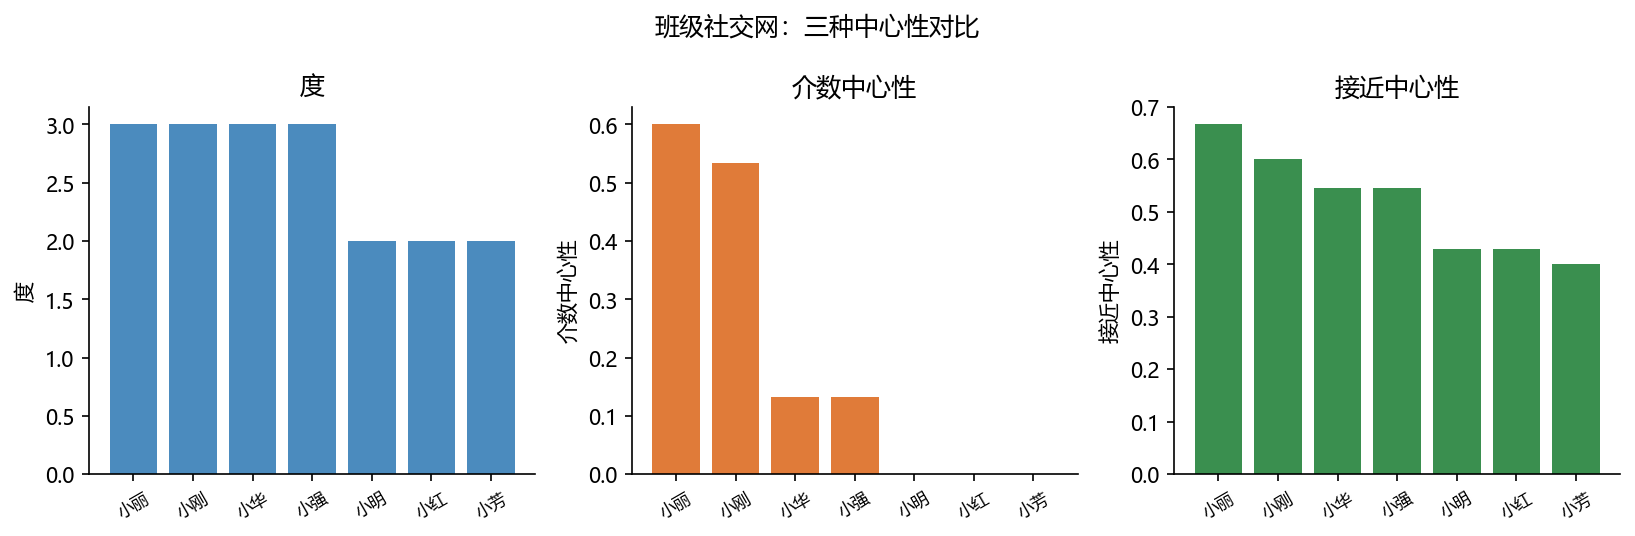
\includegraphics[keepaspectratio,alt={三种中心性对比}]{figures/06-networkx/case2_centrality.png}}
\caption{三种中心性对比}
\end{figure}

\subsubsection{主要用法 / API}\label{ux4e3bux8981ux7528ux6cd5-api-25}

{\def\LTcaptype{none} % do not increment counter
\begin{longtable}[]{@{}
  >{\raggedright\arraybackslash}p{(\linewidth - 4\tabcolsep) * \real{0.3333}}
  >{\raggedright\arraybackslash}p{(\linewidth - 4\tabcolsep) * \real{0.3333}}
  >{\raggedright\arraybackslash}p{(\linewidth - 4\tabcolsep) * \real{0.3333}}@{}}
\toprule\noalign{}
\begin{minipage}[b]{\linewidth}\raggedright
需求
\end{minipage} & \begin{minipage}[b]{\linewidth}\raggedright
写法
\end{minipage} & \begin{minipage}[b]{\linewidth}\raggedright
说明
\end{minipage} \\
\midrule\noalign{}
\endhead
\bottomrule\noalign{}
\endlastfoot
度中心性 & \texttt{nx.degree(G)} / \texttt{G.degree(node)} &
直接邻居数 \\
介数中心性 & \texttt{nx.betweenness\_centrality(G)} &
经过该点的最短路占比 \\
接近中心性 & \texttt{nx.closeness\_centrality(G)} &
平均距离越短越接近 \\
选最高 & \texttt{max(d,\ key=d.get)} 或
\texttt{sorted(d.items(),\ key=lambda\ x:\ (-x{[}1{]},\ x{[}0{]}))} &
找``最重要''节点 \\
批量画柱状图 & \texttt{plt.subplots(1,\ 3)} +
\texttt{ax.bar(names,\ vals)} & 三指标并排 \\
\end{longtable}
}

\subsubsection{常见错误}\label{ux5e38ux89c1ux9519ux8bef-25}

\begin{enumerate}
\def\labelenumi{\arabic{enumi}.}
\tightlist
\item
  以为``度最高=最重要''：本例度并列的有 4
  人，但真正扛起沟通的是介数最高的小丽。
\item
  直接 \texttt{print(nx.betweenness\_centrality(G))} 输出很多小数 →
  建议先 \texttt{round(v,\ 4)} 再打印。
\item
  用 \texttt{max(bc,\ key=bc.get)}
  只拿到``最高人''，但并列时只返回第一个；想要前三名要用
  \texttt{sorted(...){[}:3{]}}。
\item
  画条形图时不用 \texttt{sorted(C.nodes())} 固定顺序：如果直接用
  \texttt{C.nodes()} 的迭代顺序，不同环境可能顺序不同。
\end{enumerate}

\subsubsection{拓展 / 跟练}\label{ux62d3ux5c55-ux8ddfux7ec3-13}

\begin{enumerate}
\def\labelenumi{\arabic{enumi}.}
\tightlist
\item
  把小明和小芳直接连起来，观察小丽/小刚的介数如何下降。
\item
  在 \texttt{nx.karate\_club\_graph()} 上分别算三种中心性的前三名，比较
  0 号与 33 号谁更像``中心''。
\item
  用 \texttt{nx.betweenness\_centrality(G,\ k=20)} 在大图上做近似（k
  个随机源），并与精确值比较。
\item
  结合 \texttt{nx.community.greedy\_modularity\_communities}
  划分社区，再看``跨社区的桥节点''是不是就是介数最高的人。
\end{enumerate}

\begin{center}\rule{0.5\linewidth}{0.5pt}\end{center}

\subsection{常见误区}\label{ux5e38ux89c1ux8befux533a-18}

\begin{enumerate}
\def\labelenumi{\arabic{enumi}.}
\tightlist
\item
  \textbf{混淆度与中心性}：度只看``直接邻居数''，介数/接近中心性还考虑``经过该点的路径/到所有点的距离''，三者含义不同。
\item
  \textbf{在有向图上直接算
  average\_shortest\_path\_length}：默认需要图连通；若不连通，先取某个连通子图或用
  weak/strong 分量。
\item
  \textbf{把传递性当作``每个节点聚类系数的平均''}：两者定义不同（传递性按三角形/开放三元组分子分母算，平均聚类系数是各节点
  C 的均值）。
\item
  \textbf{社区划分结果不唯一}：贪心模块度算法对初始顺序、图结构敏感，Q
  只能说明``这个划分不错''，不等于``唯一正确答案''。
\item
  \textbf{计算介数中心性不限制节点数}：默认 exact
  精确算法在大图很慢；可用 k 参数抽样或只看部分节点。
\end{enumerate}

\subsection{思考题}\label{ux601dux8003ux9898-20}

\begin{enumerate}
\def\labelenumi{\arabic{enumi}.}
\tightlist
\item
  一个``星形图''（star\_graph(5)）的平均路径长度、直径、中心节点分别是什么？中心节点的介数中心性是多少？
\item
  为什么完全图（complete\_graph(10)）的平均聚类系数是 1，传递性也是 1？
\item
  给一个``连通但接近断裂''的图，哪个节点介数中心性最高？如何用代码找出``割点''？
\end{enumerate}

\subsection{动手练习（详见
lab）}\label{ux52a8ux624bux7ec3ux4e60ux8be6ux89c1-lab-12}

\begin{itemize}
\tightlist
\item
  构造
  path\_graph(8)，计算平均路径长度、直径、半径、各节点聚类系数与介数中心性；
\item
  构造两个连通分量，用 connected\_components 输出每个分量；
\item
  在 karate\_club\_graph 上分别计算 average\_clustering 与
  transitivity，比较并解释；
\item
  用 greedy\_modularity\_communities 划分 karate 网络，输出 Q
  与每个社区大小。
\end{itemize}

\subsection{延伸阅读}\label{ux5ef6ux4f38ux9605ux8bfb-27}

\begin{itemize}
\tightlist
\item
  NetworkX
  官方中心性算法：\href{https://networkx.org/documentation/stable/reference/algorithms/centrality.html}{链接}
\item
  NetworkX
  官方连通性算法：\href{https://networkx.org/documentation/stable/reference/algorithms/connectivity.html}{链接}
\item
  NetworkX
  官方社区检测：\href{https://networkx.org/documentation/stable/reference/algorithms/community.html}{链接}
\end{itemize}

\section{03
求解图的基本问题：遍历、最小生成树与最短路径}\label{ux6c42ux89e3ux56feux7684ux57faux672cux95eeux9898ux904dux5386ux6700ux5c0fux751fux6210ux6811ux4e0eux6700ux77edux8defux5f84}

\begin{quote}
本节对应原版 6.3
的内容。围绕三类经典问题：遍历（DFS/BFS）、最小生成树、最短路径。
\end{quote}

\subsection{本节目标}\label{ux672cux8282ux76eeux6807-25}

\begin{itemize}
\tightlist
\item
  会用 DFS / BFS 遍历图并得到节点访问顺序；
\item
  会用 minimum\_spanning\_tree 求解最小生成树并计算总权重；
\item
  会区分并使用 Dijkstra、Bellman-Ford、Floyd-Warshall 求解最短路径；
\item
  能根据图的特性（有权/无权、有负权/无负权、单源/全源）选择合适的算法。
\end{itemize}

\subsection{先修}\label{ux5148ux4fee-18}

\begin{itemize}
\tightlist
\item
  第 01 节：创建图、访问节点边；第 02 节：连通性概念。
\end{itemize}

\begin{center}\rule{0.5\linewidth}{0.5pt}\end{center}

\subsection{3.1 遍历问题（DFS /
BFS）}\label{ux904dux5386ux95eeux9898dfs-bfs}

\subsubsection{3.1.1
深度优先遍历（DFS）}\label{ux6df1ux5ea6ux4f18ux5148ux904dux5386dfs}

\begin{Shaded}
\begin{Highlighting}[]
\ImportTok{import}\NormalTok{ networkx }\ImportTok{as}\NormalTok{ nx}

\NormalTok{G }\OperatorTok{=}\NormalTok{ nx.Graph()}
\NormalTok{edges }\OperatorTok{=}\NormalTok{ [(}\DecValTok{1}\NormalTok{, }\DecValTok{2}\NormalTok{), (}\DecValTok{1}\NormalTok{, }\DecValTok{3}\NormalTok{), (}\DecValTok{2}\NormalTok{, }\DecValTok{4}\NormalTok{), (}\DecValTok{3}\NormalTok{, }\DecValTok{4}\NormalTok{), (}\DecValTok{4}\NormalTok{, }\DecValTok{5}\NormalTok{)]}
\NormalTok{G.add\_edges\_from(edges)}

\NormalTok{start\_node }\OperatorTok{=} \DecValTok{1}
\NormalTok{visited }\OperatorTok{=} \BuiltInTok{list}\NormalTok{(nx.dfs\_preorder\_nodes(G, start\_node))}
\BuiltInTok{print}\NormalTok{(}\StringTok{"DFS 遍历顺序:"}\NormalTok{, visited)}
\BuiltInTok{print}\NormalTok{(}\StringTok{"DFS 边:"}\NormalTok{, }\BuiltInTok{list}\NormalTok{(nx.dfs\_edges(G, start\_node)))}
\end{Highlighting}
\end{Shaded}

\begin{Shaded}
\begin{Highlighting}[]
\NormalTok{DFS 遍历顺序: [1, 2, 4, 3, 5]}
\NormalTok{DFS 边: [(1, 2), (2, 4), (4, 3), (4, 5)]}
\end{Highlighting}
\end{Shaded}

\subsubsection{3.1.2
广度优先遍历（BFS）}\label{ux5e7fux5ea6ux4f18ux5148ux904dux5386bfs}

bfs\_edges 返回按广度扩展的边，可由此构建节点访问顺序：

\begin{Shaded}
\begin{Highlighting}[]
\BuiltInTok{print}\NormalTok{(}\StringTok{"BFS 边:"}\NormalTok{, }\BuiltInTok{list}\NormalTok{(nx.bfs\_edges(G, start\_node)))}
\BuiltInTok{print}\NormalTok{(}\StringTok{"BFS 树边:"}\NormalTok{, }\BuiltInTok{list}\NormalTok{(nx.bfs\_tree(G, start\_node).edges()))}

\CommentTok{\#\# 用集合去重 + 列表保持顺序}
\NormalTok{seen }\OperatorTok{=} \BuiltInTok{set}\NormalTok{()}
\NormalTok{bfs\_order }\OperatorTok{=}\NormalTok{ []}
\ControlFlowTok{for}\NormalTok{ u, v }\KeywordTok{in}\NormalTok{ nx.bfs\_edges(G, start\_node):}
    \ControlFlowTok{if}\NormalTok{ u }\KeywordTok{not} \KeywordTok{in}\NormalTok{ seen:}
\NormalTok{        seen.add(u)}\OperatorTok{;}\NormalTok{ bfs\_order.append(u)}
    \ControlFlowTok{if}\NormalTok{ v }\KeywordTok{not} \KeywordTok{in}\NormalTok{ seen:}
\NormalTok{        seen.add(v)}\OperatorTok{;}\NormalTok{ bfs\_order.append(v)}
\BuiltInTok{print}\NormalTok{(}\StringTok{"BFS 节点顺序:"}\NormalTok{, bfs\_order)}
\end{Highlighting}
\end{Shaded}

\begin{Shaded}
\begin{Highlighting}[]
\NormalTok{BFS 边: [(1, 2), (1, 3), (2, 4), (4, 5)]}
\NormalTok{BFS 树边: [(1, 2), (1, 3), (2, 4), (4, 5)]}
\NormalTok{BFS 节点顺序: [1, 2, 3, 4, 5]}
\end{Highlighting}
\end{Shaded}

\begin{quote}
DFS 优先``一条路走到黑''，BFS 按``层''逐层扩散。在无权图上，BFS
得到的路径就是最短路径（边数最少）。
\end{quote}

\begin{center}\rule{0.5\linewidth}{0.5pt}\end{center}

\subsection{3.2 最小生成树（Minimum Spanning Tree,
MST）}\label{ux6700ux5c0fux751fux6210ux6811minimum-spanning-tree-mst}

\subsubsection{3.2.1 问题}\label{ux95eeux9898}

给定一个加权无向连通图，找到一棵边的总权重最小的生成树（连接所有节点且无环）。NetworkX
提供 minimum\_spanning\_tree，默认用 Kruskal
算法（适合稀疏图）；稠密图可考虑 Prim 思想，但官方没有直接的 Prim
选项，多数场景 Kruskal 已足够。

\begin{Shaded}
\begin{Highlighting}[]
\NormalTok{G }\OperatorTok{=}\NormalTok{ nx.Graph()}
\NormalTok{edges }\OperatorTok{=}\NormalTok{ [}
\NormalTok{    (}\StringTok{"A"}\NormalTok{, }\StringTok{"B"}\NormalTok{, }\DecValTok{10}\NormalTok{),}
\NormalTok{    (}\StringTok{"A"}\NormalTok{, }\StringTok{"C"}\NormalTok{, }\DecValTok{6}\NormalTok{),}
\NormalTok{    (}\StringTok{"A"}\NormalTok{, }\StringTok{"D"}\NormalTok{, }\DecValTok{5}\NormalTok{),}
\NormalTok{    (}\StringTok{"B"}\NormalTok{, }\StringTok{"C"}\NormalTok{, }\DecValTok{5}\NormalTok{),}
\NormalTok{    (}\StringTok{"B"}\NormalTok{, }\StringTok{"D"}\NormalTok{, }\DecValTok{15}\NormalTok{),}
\NormalTok{    (}\StringTok{"B"}\NormalTok{, }\StringTok{"E"}\NormalTok{, }\DecValTok{4}\NormalTok{),}
\NormalTok{    (}\StringTok{"C"}\NormalTok{, }\StringTok{"D"}\NormalTok{, }\DecValTok{15}\NormalTok{),}
\NormalTok{    (}\StringTok{"C"}\NormalTok{, }\StringTok{"F"}\NormalTok{, }\DecValTok{12}\NormalTok{),}
\NormalTok{    (}\StringTok{"D"}\NormalTok{, }\StringTok{"E"}\NormalTok{, }\DecValTok{20}\NormalTok{),}
\NormalTok{    (}\StringTok{"E"}\NormalTok{, }\StringTok{"F"}\NormalTok{, }\DecValTok{9}\NormalTok{),}
\NormalTok{]}
\NormalTok{G.add\_weighted\_edges\_from(edges)}

\NormalTok{T }\OperatorTok{=}\NormalTok{ nx.minimum\_spanning\_tree(G)}

\BuiltInTok{print}\NormalTok{(}\StringTok{"MST 边："}\NormalTok{)}
\ControlFlowTok{for}\NormalTok{ u, v, weight }\KeywordTok{in}\NormalTok{ T.edges(data}\OperatorTok{=}\StringTok{"weight"}\NormalTok{):}
    \BuiltInTok{print}\NormalTok{(u, }\StringTok{"{-}{-}"}\NormalTok{, v, }\StringTok{"weighted"}\NormalTok{, weight)}
\BuiltInTok{print}\NormalTok{(}\StringTok{"MST 总权重:"}\NormalTok{, }\BuiltInTok{sum}\NormalTok{(w }\ControlFlowTok{for}\NormalTok{ \_, \_, w }\KeywordTok{in}\NormalTok{ T.edges(data}\OperatorTok{=}\StringTok{"weight"}\NormalTok{)))}
\BuiltInTok{print}\NormalTok{(}\StringTok{"MST 边数:"}\NormalTok{, T.number\_of\_edges())}
\end{Highlighting}
\end{Shaded}

\begin{Shaded}
\begin{Highlighting}[]
\NormalTok{MST 边：}
\NormalTok{A {-}{-} D weighted 5}
\NormalTok{A {-}{-} C weighted 6}
\NormalTok{B {-}{-} E weighted 4}
\NormalTok{B {-}{-} C weighted 5}
\NormalTok{E {-}{-} F weighted 9}
\NormalTok{MST 总权重: 29}
\NormalTok{MST 边数: 5}
\end{Highlighting}
\end{Shaded}

\begin{quote}
选择边 \{B-E(4), A-D(5), B-C(5), A-C(6), E-F(9)\}，总权重 29；连通
A、B、C、D、E、F 且无环。
\end{quote}

\begin{center}\rule{0.5\linewidth}{0.5pt}\end{center}

\subsection{3.3
最短路径问题}\label{ux6700ux77edux8defux5f84ux95eeux9898}

\subsubsection{3.3.1 Dijkstra
算法（非负权、单源）}\label{dijkstra-ux7b97ux6cd5ux975eux8d1fux6743ux5355ux6e90}

适用于边权非负的图。用 dijkstra\_path 求路径，dijkstra\_path\_length
求长度。

\begin{Shaded}
\begin{Highlighting}[]
\NormalTok{DG }\OperatorTok{=}\NormalTok{ nx.DiGraph()}
\NormalTok{DG.add\_edge(}\StringTok{"A"}\NormalTok{, }\StringTok{"B"}\NormalTok{, weight}\OperatorTok{=}\DecValTok{3}\NormalTok{)}
\NormalTok{DG.add\_edge(}\StringTok{"A"}\NormalTok{, }\StringTok{"C"}\NormalTok{, weight}\OperatorTok{=}\DecValTok{2}\NormalTok{)}
\NormalTok{DG.add\_edge(}\StringTok{"B"}\NormalTok{, }\StringTok{"C"}\NormalTok{, weight}\OperatorTok{=}\DecValTok{1}\NormalTok{)}
\NormalTok{DG.add\_edge(}\StringTok{"B"}\NormalTok{, }\StringTok{"D"}\NormalTok{, weight}\OperatorTok{=}\DecValTok{4}\NormalTok{)}
\NormalTok{DG.add\_edge(}\StringTok{"C"}\NormalTok{, }\StringTok{"D"}\NormalTok{, weight}\OperatorTok{=}\DecValTok{2}\NormalTok{)}
\NormalTok{DG.add\_edge(}\StringTok{"C"}\NormalTok{, }\StringTok{"E"}\NormalTok{, weight}\OperatorTok{=}\DecValTok{1}\NormalTok{)}
\NormalTok{DG.add\_edge(}\StringTok{"D"}\NormalTok{, }\StringTok{"E"}\NormalTok{, weight}\OperatorTok{=}\DecValTok{3}\NormalTok{)}

\NormalTok{shortest\_path }\OperatorTok{=}\NormalTok{ nx.dijkstra\_path(DG, }\StringTok{"A"}\NormalTok{, }\StringTok{"E"}\NormalTok{, weight}\OperatorTok{=}\StringTok{"weight"}\NormalTok{)}
\NormalTok{shortest\_length }\OperatorTok{=}\NormalTok{ nx.dijkstra\_path\_length(DG, }\StringTok{"A"}\NormalTok{, }\StringTok{"E"}\NormalTok{, weight}\OperatorTok{=}\StringTok{"weight"}\NormalTok{)}
\BuiltInTok{print}\NormalTok{(}\StringTok{"最短路径:"}\NormalTok{, shortest\_path)}
\BuiltInTok{print}\NormalTok{(}\StringTok{"最短路径长度:"}\NormalTok{, shortest\_length)}

\CommentTok{\#\# 从 A 到所有点的最短距离}
\BuiltInTok{print}\NormalTok{(}\StringTok{"单源最短路径长度:"}\NormalTok{, nx.single\_source\_dijkstra\_path\_length(DG, }\StringTok{"A"}\NormalTok{, weight}\OperatorTok{=}\StringTok{"weight"}\NormalTok{))}
\end{Highlighting}
\end{Shaded}

\begin{Shaded}
\begin{Highlighting}[]
\NormalTok{最短路径: [\textquotesingle{}A\textquotesingle{}, \textquotesingle{}C\textquotesingle{}, \textquotesingle{}E\textquotesingle{}]}
\NormalTok{最短路径长度: 3}
\NormalTok{单源最短路径长度: \{\textquotesingle{}A\textquotesingle{}: 0, \textquotesingle{}C\textquotesingle{}: 2, \textquotesingle{}B\textquotesingle{}: 3, \textquotesingle{}E\textquotesingle{}: 3, \textquotesingle{}D\textquotesingle{}: 4\}}
\end{Highlighting}
\end{Shaded}

注意：从 A 到 E 走 A→C→E 是 2+1=3，比 A→B→C→E（3+1+1=5）和
A→C→D→E（2+2+3=7）都短。

\subsubsection{3.3.2 Bellman-Ford
算法（可处理负权边、单源）}\label{bellman-ford-ux7b97ux6cd5ux53efux5904ux7406ux8d1fux6743ux8fb9ux5355ux6e90}

当图中存在负权边（但没有负权回路）时，Dijkstra 不再适用，可用
Bellman-Ford。时间复杂度 O(VE)。

\begin{Shaded}
\begin{Highlighting}[]
\BuiltInTok{print}\NormalTok{(}\StringTok{"Bellman{-}Ford 路径:"}\NormalTok{, nx.bellman\_ford\_path(DG, }\StringTok{"A"}\NormalTok{, }\StringTok{"E"}\NormalTok{, weight}\OperatorTok{=}\StringTok{"weight"}\NormalTok{))}
\BuiltInTok{print}\NormalTok{(}\StringTok{"Bellman{-}Ford 长度:"}\NormalTok{, nx.bellman\_ford\_path\_length(DG, }\StringTok{"A"}\NormalTok{, }\StringTok{"E"}\NormalTok{, weight}\OperatorTok{=}\StringTok{"weight"}\NormalTok{))}
\end{Highlighting}
\end{Shaded}

\begin{Shaded}
\begin{Highlighting}[]
\NormalTok{Bellman{-}Ford 路径: [\textquotesingle{}A\textquotesingle{}, \textquotesingle{}C\textquotesingle{}, \textquotesingle{}E\textquotesingle{}]}
\NormalTok{Bellman{-}Ford 长度: 3}
\end{Highlighting}
\end{Shaded}

\subsubsection{3.3.3 Floyd-Warshall
算法（全源最短路径）}\label{floyd-warshall-ux7b97ux6cd5ux5168ux6e90ux6700ux77edux8defux5f84}

需要``所有点对之间的最短距离''时用 Floyd-Warshall，O(V\^{}3)。networkx
提供 floyd\_warshall / floyd\_warshall\_numpy。

\begin{Shaded}
\begin{Highlighting}[]
\ImportTok{import}\NormalTok{ numpy }\ImportTok{as}\NormalTok{ np}
\NormalTok{path\_lengths }\OperatorTok{=}\NormalTok{ nx.floyd\_warshall\_numpy(DG, weight}\OperatorTok{=}\StringTok{"weight"}\NormalTok{)}
\BuiltInTok{print}\NormalTok{(}\StringTok{"矩阵形状:"}\NormalTok{, path\_lengths.shape)}
\NormalTok{idx }\OperatorTok{=} \BuiltInTok{list}\NormalTok{(DG.nodes())}
\NormalTok{iA }\OperatorTok{=}\NormalTok{ idx.index(}\StringTok{"A"}\NormalTok{)}\OperatorTok{;}\NormalTok{ iE }\OperatorTok{=}\NormalTok{ idx.index(}\StringTok{"E"}\NormalTok{)}
\BuiltInTok{print}\NormalTok{(}\StringTok{"A 到 E 的距离:"}\NormalTok{, path\_lengths[iA, iE])}
\BuiltInTok{print}\NormalTok{(}\StringTok{"A 行:"}\NormalTok{, path\_lengths[iA, :])}
\end{Highlighting}
\end{Shaded}

\begin{Shaded}
\begin{Highlighting}[]
\NormalTok{矩阵形状: (5, 5)}
\NormalTok{A 到 E 的距离: 3.0}
\NormalTok{A 行: [0. 3. 2. 4. 3.]}
\end{Highlighting}
\end{Shaded}

\begin{quote}
Floyd-Warshall 不直接返回路径；若需要路径，可结合 shortest\_path
逐步重建，或用 nx.shortest\_path(G, source, target, weight=``weight'')
得到一条具体路径。
\end{quote}

\subsubsection{3.3.4
算法选择速查}\label{ux7b97ux6cd5ux9009ux62e9ux901fux67e5}

{\def\LTcaptype{none} % do not increment counter
\begin{longtable}[]{@{}
  >{\raggedright\arraybackslash}p{(\linewidth - 6\tabcolsep) * \real{0.2500}}
  >{\raggedright\arraybackslash}p{(\linewidth - 6\tabcolsep) * \real{0.2500}}
  >{\raggedright\arraybackslash}p{(\linewidth - 6\tabcolsep) * \real{0.2500}}
  >{\raggedright\arraybackslash}p{(\linewidth - 6\tabcolsep) * \real{0.2500}}@{}}
\toprule\noalign{}
\begin{minipage}[b]{\linewidth}\raggedright
需求
\end{minipage} & \begin{minipage}[b]{\linewidth}\raggedright
图特性
\end{minipage} & \begin{minipage}[b]{\linewidth}\raggedright
推荐函数
\end{minipage} & \begin{minipage}[b]{\linewidth}\raggedright
复杂度
\end{minipage} \\
\midrule\noalign{}
\endhead
\bottomrule\noalign{}
\endlastfoot
单源、非负权 & 无负权 & dijkstra\_path / dijkstra\_path\_length &
O((V+E) log V) \\
单源、可能有负权 & 允许负权但无负环 & bellman\_ford\_path & O(VE) \\
全源最短距离 & 可含负权（无负环） & floyd\_warshall /
floyd\_warshall\_numpy & O(V\^{}3) \\
无权最短路径 & 边权都为 1 & shortest\_path / bfs & O(V+E) \\
\end{longtable}
}

\subsection{案例卡
3：加权最短路径------地铁换乘总时间最少路线}\label{ux6848ux4f8bux5361-3ux52a0ux6743ux6700ux77edux8defux5f84ux5730ux94c1ux6362ux4e58ux603bux65f6ux95f4ux6700ux5c11ux8defux7ebf}

\subsubsection{目标}\label{ux76eeux6807-26}

把地铁站当节点、站间行驶时间(分钟)当\textbf{边权}，用
\texttt{nx.dijkstra\_path}
求``从中央公园到科技园''总时间最少的换乘路线，并打印从起点到所有站的最少时间。这是``带权图上找最短路''的典型应用。

\subsubsection{代码}\label{ux4ee3ux7801-27}

\begin{Shaded}
\begin{Highlighting}[]
\ImportTok{import}\NormalTok{ networkx }\ImportTok{as}\NormalTok{ nx}
\ImportTok{import}\NormalTok{ matplotlib.pyplot }\ImportTok{as}\NormalTok{ plt}
\ImportTok{import}\NormalTok{ numpy }\ImportTok{as}\NormalTok{ np}
\ImportTok{import}\NormalTok{ os}

\NormalTok{plt.rcParams[}\StringTok{\textquotesingle{}font.sans{-}serif\textquotesingle{}}\NormalTok{] }\OperatorTok{=}\NormalTok{ [}\StringTok{\textquotesingle{}Microsoft YaHei\textquotesingle{}}\NormalTok{, }\StringTok{\textquotesingle{}SimHei\textquotesingle{}}\NormalTok{, }\StringTok{\textquotesingle{}DejaVu Sans\textquotesingle{}}\NormalTok{]}
\NormalTok{plt.rcParams[}\StringTok{\textquotesingle{}axes.unicode\_minus\textquotesingle{}}\NormalTok{] }\OperatorTok{=} \VariableTok{False}
\NormalTok{np.set\_printoptions(precision}\OperatorTok{=}\DecValTok{4}\NormalTok{, suppress}\OperatorTok{=}\VariableTok{True}\NormalTok{)}

\CommentTok{\#\# 1) 地铁网：节点=车站，边的 weight=行驶分钟(双向)}
\NormalTok{M }\OperatorTok{=}\NormalTok{ nx.Graph()}
\NormalTok{M.add\_weighted\_edges\_from([}
\NormalTok{    (}\StringTok{\textquotesingle{}中央公园\textquotesingle{}}\NormalTok{,}\StringTok{\textquotesingle{}城东\textquotesingle{}}\NormalTok{, }\DecValTok{3}\NormalTok{), (}\StringTok{\textquotesingle{}中央公园\textquotesingle{}}\NormalTok{,}\StringTok{\textquotesingle{}大学城\textquotesingle{}}\NormalTok{, }\DecValTok{2}\NormalTok{),}
\NormalTok{    (}\StringTok{\textquotesingle{}城东\textquotesingle{}}\NormalTok{,}\StringTok{\textquotesingle{}大学城\textquotesingle{}}\NormalTok{, }\DecValTok{1}\NormalTok{), (}\StringTok{\textquotesingle{}城东\textquotesingle{}}\NormalTok{,}\StringTok{\textquotesingle{}火车站\textquotesingle{}}\NormalTok{, }\DecValTok{4}\NormalTok{), (}\StringTok{\textquotesingle{}大学城\textquotesingle{}}\NormalTok{,}\StringTok{\textquotesingle{}火车站\textquotesingle{}}\NormalTok{, }\DecValTok{2}\NormalTok{),}
\NormalTok{    (}\StringTok{\textquotesingle{}大学城\textquotesingle{}}\NormalTok{,}\StringTok{\textquotesingle{}机场\textquotesingle{}}\NormalTok{, }\DecValTok{1}\NormalTok{), (}\StringTok{\textquotesingle{}火车站\textquotesingle{}}\NormalTok{,}\StringTok{\textquotesingle{}机场\textquotesingle{}}\NormalTok{, }\DecValTok{3}\NormalTok{), (}\StringTok{\textquotesingle{}火车站\textquotesingle{}}\NormalTok{,}\StringTok{\textquotesingle{}科技园\textquotesingle{}}\NormalTok{, }\DecValTok{2}\NormalTok{), (}\StringTok{\textquotesingle{}机场\textquotesingle{}}\NormalTok{,}\StringTok{\textquotesingle{}科技园\textquotesingle{}}\NormalTok{, }\DecValTok{4}\NormalTok{),}
\NormalTok{])}

\CommentTok{\#\# 2) Dijkstra：单源最短路径/长度(默认按边权)}
\NormalTok{path }\OperatorTok{=}\NormalTok{ nx.dijkstra\_path(M, }\StringTok{\textquotesingle{}中央公园\textquotesingle{}}\NormalTok{, }\StringTok{\textquotesingle{}科技园\textquotesingle{}}\NormalTok{, weight}\OperatorTok{=}\StringTok{\textquotesingle{}weight\textquotesingle{}}\NormalTok{)}
\NormalTok{length }\OperatorTok{=}\NormalTok{ nx.dijkstra\_path\_length(M, }\StringTok{\textquotesingle{}中央公园\textquotesingle{}}\NormalTok{, }\StringTok{\textquotesingle{}科技园\textquotesingle{}}\NormalTok{, weight}\OperatorTok{=}\StringTok{\textquotesingle{}weight\textquotesingle{}}\NormalTok{)}
\BuiltInTok{print}\NormalTok{(}\StringTok{\textquotesingle{}最短路径:\textquotesingle{}}\NormalTok{, path)}
\BuiltInTok{print}\NormalTok{(}\StringTok{\textquotesingle{}最短时间(分钟):\textquotesingle{}}\NormalTok{, length)}

\CommentTok{\#\# 3) 从起点到所有站的最少时间(按站名排序保证顺序稳定)}
\NormalTok{sdd }\OperatorTok{=}\NormalTok{ nx.single\_source\_dijkstra\_path\_length(M, }\StringTok{\textquotesingle{}中央公园\textquotesingle{}}\NormalTok{, weight}\OperatorTok{=}\StringTok{\textquotesingle{}weight\textquotesingle{}}\NormalTok{)}
\BuiltInTok{print}\NormalTok{(}\StringTok{\textquotesingle{}单源最短时间(按站名排序):\textquotesingle{}}\NormalTok{, \{k: }\BuiltInTok{round}\NormalTok{(v, }\DecValTok{4}\NormalTok{) }\ControlFlowTok{for}\NormalTok{ k, v }\KeywordTok{in} \BuiltInTok{sorted}\NormalTok{(sdd.items())\})}

\CommentTok{\#\# 4) 把最短路线画出来}
\NormalTok{path\_edges }\OperatorTok{=} \BuiltInTok{list}\NormalTok{(}\BuiltInTok{zip}\NormalTok{(path[:}\OperatorTok{{-}}\DecValTok{1}\NormalTok{], path[}\DecValTok{1}\NormalTok{:]))}
\NormalTok{pos }\OperatorTok{=}\NormalTok{ nx.spring\_layout(M, seed}\OperatorTok{=}\DecValTok{42}\NormalTok{, k}\OperatorTok{=}\FloatTok{0.9}\NormalTok{)}
\NormalTok{os.makedirs(}\StringTok{\textquotesingle{}images\textquotesingle{}}\NormalTok{, exist\_ok}\OperatorTok{=}\VariableTok{True}\NormalTok{)}
\NormalTok{plt.figure(figsize}\OperatorTok{=}\NormalTok{(}\FloatTok{7.0}\NormalTok{, }\FloatTok{5.0}\NormalTok{))}
\NormalTok{nx.draw\_networkx\_nodes(M, pos, node\_size}\OperatorTok{=}\DecValTok{650}\NormalTok{, node\_color}\OperatorTok{=}\StringTok{\textquotesingle{}\#dff3e0\textquotesingle{}}\NormalTok{, edgecolors}\OperatorTok{=}\StringTok{\textquotesingle{}\#3a8f4f\textquotesingle{}}\NormalTok{)}
\NormalTok{nx.draw\_networkx\_edges(M, pos, alpha}\OperatorTok{=}\FloatTok{0.35}\NormalTok{, edge\_color}\OperatorTok{=}\StringTok{\textquotesingle{}\#999999\textquotesingle{}}\NormalTok{, width}\OperatorTok{=}\FloatTok{1.2}\NormalTok{)}
\NormalTok{nx.draw\_networkx\_edges(M, pos, edgelist}\OperatorTok{=}\NormalTok{path\_edges, edge\_color}\OperatorTok{=}\StringTok{\textquotesingle{}\#c0392b\textquotesingle{}}\NormalTok{, width}\OperatorTok{=}\FloatTok{3.0}\NormalTok{)}
\NormalTok{nx.draw\_networkx\_labels(M, pos, font\_size}\OperatorTok{=}\DecValTok{11}\NormalTok{, font\_family}\OperatorTok{=}\StringTok{\textquotesingle{}Microsoft YaHei\textquotesingle{}}\NormalTok{)}
\NormalTok{plt.title(}\StringTok{\textquotesingle{}地铁网：中央公园 {-}\textgreater{} 科技园 最少时间路线\textquotesingle{}}\NormalTok{)}
\NormalTok{plt.axis(}\StringTok{\textquotesingle{}off\textquotesingle{}}\NormalTok{)}
\NormalTok{plt.tight\_layout()}
\NormalTok{plt.savefig(}\StringTok{\textquotesingle{}figures/06{-}networkx/case3\_metro.png\textquotesingle{}}\NormalTok{, dpi}\OperatorTok{=}\DecValTok{150}\NormalTok{)}
\BuiltInTok{print}\NormalTok{(}\StringTok{\textquotesingle{}已保存 figures/06{-}networkx/case3\_metro.png\textquotesingle{}}\NormalTok{)}
\NormalTok{plt.close()}
\end{Highlighting}
\end{Shaded}

\subsubsection{运行结果(已运行核验)}\label{ux8fd0ux884cux7ed3ux679cux5df2ux8fd0ux884cux6838ux9a8c-25}

\begin{Shaded}
\begin{Highlighting}[]
\NormalTok{最短路径: [\textquotesingle{}中央公园\textquotesingle{}, \textquotesingle{}大学城\textquotesingle{}, \textquotesingle{}火车站\textquotesingle{}, \textquotesingle{}科技园\textquotesingle{}]}
\NormalTok{最短时间(分钟): 6}
\NormalTok{单源最短时间(按站名排序): \{\textquotesingle{}中央公园\textquotesingle{}: 0, \textquotesingle{}城东\textquotesingle{}: 3, \textquotesingle{}大学城\textquotesingle{}: 2, \textquotesingle{}机场\textquotesingle{}: 3, \textquotesingle{}火车站\textquotesingle{}: 4, \textquotesingle{}科技园\textquotesingle{}: 6\}}
\NormalTok{已保存 figures/06{-}networkx/case3\_metro.png}
\end{Highlighting}
\end{Shaded}

\subsubsection{讲解}\label{ux8bb2ux89e3-25}

\textbf{一句话解释}：每条地铁线都标上``坐多久''，Dijkstra
就会像贪心一样从起点出发，每次先挑``目前累计时间最少''的站往前扩，最后得到总时间最少的换乘方案。

\begin{enumerate}
\def\labelenumi{\arabic{enumi}.}
\tightlist
\item
  \texttt{M.add\_weighted\_edges\_from(...)} 每条边的 \texttt{weight}
  就是行驶分钟；地铁双向能坐，所以用无向 \texttt{nx.Graph} 即可。
\item
  \texttt{nx.dijkstra\_path(M,\ \textquotesingle{}中央公园\textquotesingle{},\ \textquotesingle{}科技园\textquotesingle{},\ weight=\textquotesingle{}weight\textquotesingle{})}
  返回\textbf{一条}路径
  \texttt{{[}\textquotesingle{}中央公园\textquotesingle{},\textquotesingle{}大学城\textquotesingle{},\textquotesingle{}火车站\textquotesingle{},\textquotesingle{}科技园\textquotesingle{}{]}}，时间是
  2+2+2=6 分钟。
\item
  \texttt{nx.dijkstra\_path\_length(...)} 只返回总时间
  6；\texttt{nx.single\_source\_dijkstra\_path\_length(...)}
  返回从起点到\textbf{每个站}的最少时间，例如到机场 3 分钟（经大学城
  2+1），到火车站 4 分钟（经大学城 2+2）。
\item
  注意 \texttt{weight=\textquotesingle{}weight\textquotesingle{}}
  不能漏：如果不传，NetworkX 默认把所有边权当成
  1，那就变成``换乘站数最少''，结果会不一样。
\item
  为什么走``中央公园→大学城→火车站→科技园''而不是``机场→科技园''那条？因为机场-科技园要
  4 分钟，而大学城-机场只要 1+3=4 分钟，两者到科技园都 4
  分钟；但走大学城-火车站-科技园是 2+2=4 分钟，所以整体最短是 6 分钟。
\item
  绘图用 \texttt{spring\_layout(...,\ seed=42)}
  固定布局，红色高亮最短路径；\texttt{os.makedirs(\textquotesingle{}images\textquotesingle{},\ exist\_ok=True)}
  保证目录存在。
\end{enumerate}

\begin{figure}
\centering
\pandocbounded{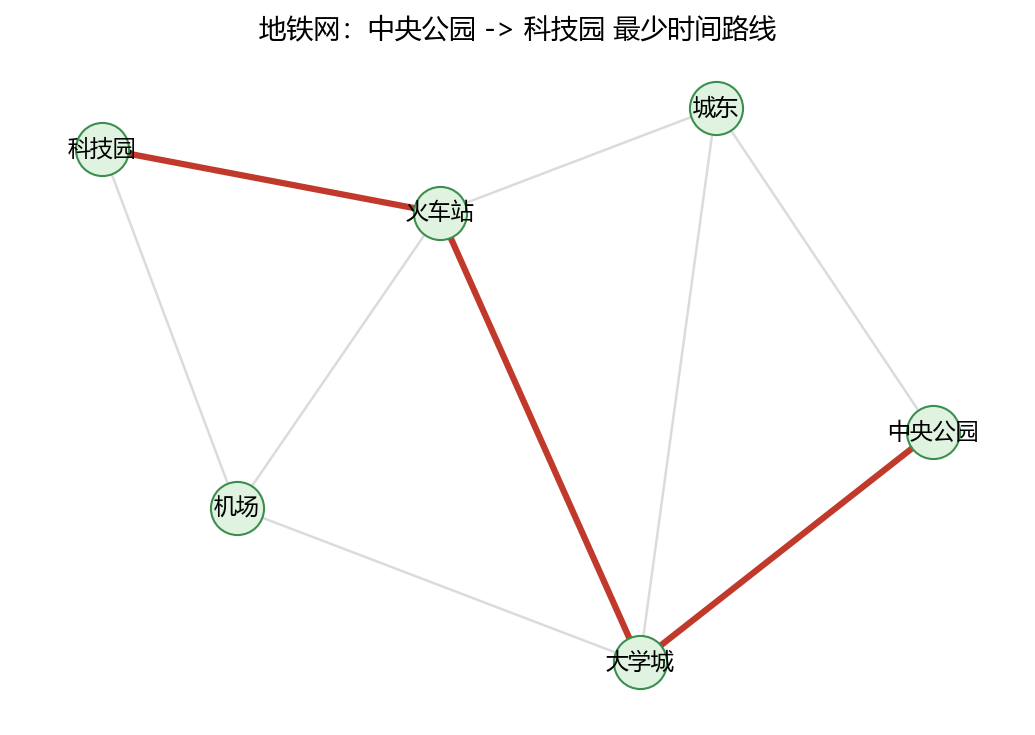
\includegraphics[keepaspectratio,alt={地铁最少时间路线}]{figures/06-networkx/case3_metro.png}}
\caption{地铁最少时间路线}
\end{figure}

\subsubsection{主要用法 / API}\label{ux4e3bux8981ux7528ux6cd5-api-26}

{\def\LTcaptype{none} % do not increment counter
\begin{longtable}[]{@{}
  >{\raggedright\arraybackslash}p{(\linewidth - 4\tabcolsep) * \real{0.3333}}
  >{\raggedright\arraybackslash}p{(\linewidth - 4\tabcolsep) * \real{0.3333}}
  >{\raggedright\arraybackslash}p{(\linewidth - 4\tabcolsep) * \real{0.3333}}@{}}
\toprule\noalign{}
\begin{minipage}[b]{\linewidth}\raggedright
需求
\end{minipage} & \begin{minipage}[b]{\linewidth}\raggedright
写法
\end{minipage} & \begin{minipage}[b]{\linewidth}\raggedright
说明
\end{minipage} \\
\midrule\noalign{}
\endhead
\bottomrule\noalign{}
\endlastfoot
加带权边 & \texttt{add\_weighted\_edges\_from({[}(u,\ v,\ w){]})} &
属性名 \texttt{weight} \\
单源最短路 &
\texttt{nx.dijkstra\_path(G,\ s,\ t,\ weight=\textquotesingle{}weight\textquotesingle{})}
& 返回一条路径 \\
最短距离 &
\texttt{nx.dijkstra\_path\_length(G,\ s,\ t,\ weight=\textquotesingle{}weight\textquotesingle{})}
& 返回总权重 \\
到所有点距离 &
\texttt{nx.single\_source\_dijkstra\_path\_length(G,\ s,\ weight=\textquotesingle{}weight\textquotesingle{})}
& 返回 dict \\
全源距离矩阵 &
\texttt{nx.floyd\_warshall\_numpy(G,\ weight=\textquotesingle{}weight\textquotesingle{})}
& 任意两点距离 \\
有负权边 &
\texttt{nx.bellman\_ford\_path(G,\ s,\ t,\ weight=\textquotesingle{}weight\textquotesingle{})}
& 改用 Bellman-Ford \\
\end{longtable}
}

\subsubsection{常见错误}\label{ux5e38ux89c1ux9519ux8bef-26}

\begin{enumerate}
\def\labelenumi{\arabic{enumi}.}
\tightlist
\item
  忘了
  \texttt{weight=\textquotesingle{}weight\textquotesingle{}}：带权图会被当成无权图，结果变成``换乘/站数最少''而不是``时间最少''。
\item
  在含负权边的图上用 Dijkstra：Dijkstra
  假设非负权；有负权（无负环）时应改用 \texttt{bellman\_ford\_path} 或
  \texttt{floyd\_warshall}。
\item
  \texttt{single\_source\_dijkstra\_path\_length} 返回的 dict 顺序不确定
  → 打印前用 \texttt{sorted(d.items())} 固定。
\item
  以为``总时间最少''等价于``经过站最少''：本例最短时间路线是 4 站 3
  段；但若把机场-科技园改成 1 分钟，最短时间路线就变成经机场的 3
  段，与少换乘目标不同。
\end{enumerate}

\subsubsection{拓展 / 跟练}\label{ux62d3ux5c55-ux8ddfux7ec3-14}

\begin{enumerate}
\def\labelenumi{\arabic{enumi}.}
\tightlist
\item
  新增一条``机场-城东''直达线(2
  分钟)，重新计算最短路与最短时间，看是否变短。
\item
  用
  \texttt{nx.shortest\_path(M,\ \textquotesingle{}中央公园\textquotesingle{},\ \textquotesingle{}科技园\textquotesingle{})}(不带
  weight)对比``站数最少''与``时间最少''两条路线。
\item
  把权重视为``票价''，用 \texttt{nx.bellman\_ford\_path}
  重算（本例无负权，结果应一致）。
\item
  用
  \texttt{nx.floyd\_warshall\_numpy(M,\ weight=\textquotesingle{}weight\textquotesingle{})}
  输出 6x6 距离矩阵，并验证对角元为 0。
\end{enumerate}

\begin{center}\rule{0.5\linewidth}{0.5pt}\end{center}

\subsection{常见误区}\label{ux5e38ux89c1ux8befux533a-19}

\begin{enumerate}
\def\labelenumi{\arabic{enumi}.}
\tightlist
\item
  \textbf{在无权图上用 Dijkstra 还传 weight=``weight''}：无权图没有
  weight 属性，直接用 shortest\_path / bfs 即可，或明确传 weight=None。
\item
  \textbf{在有负权边的图上用 Dijkstra}：Dijkstra
  假设非负权，负权会给出错误结果，应改用 Bellman-Ford。
\item
  \textbf{对不连通图调用 diameter /
  average\_shortest\_path\_length}：会抛错，先检查连通性或用连通分量分别计算。
\item
  \textbf{把 minimum\_spanning\_tree 的边权当成``路径权重''}：MST
  是为了连通所有节点总权重最小，与最短路径目标不同；两者不能混用。
\item
  \textbf{忘记 graph 需要连通才能有 MST}：minimum\_spanning\_tree
  要求输入连通（或每个分量各自生成森林）。
\end{enumerate}

\subsection{思考题}\label{ux601dux8003ux9898-21}

\begin{enumerate}
\def\labelenumi{\arabic{enumi}.}
\tightlist
\item
  BFS 在无权图上求出的路径是最短的吗？为什么？
\item
  最小生成树与最短路径有何区别？一个是``连所有点''，一个是``两点之间距离''。
\item
  对于含负权边的有向图，Floyd-Warshall
  能否给出正确答案？什么情况下会失败？
\end{enumerate}

\subsection{动手练习（详见
lab）}\label{ux52a8ux624bux7ec3ux4e60ux8be6ux89c1-lab-13}

\begin{itemize}
\tightlist
\item
  构造 path\_graph(8)，从节点 0 出发分别用 DFS、BFS 输出顺序，比较差异；
\item
  构造上面的加权图，用 minimum\_spanning\_tree 求 MST，并验证总权重=29；
\item
  构造带负权边的图，比较 Dijkstra 与 Bellman-Ford 的结果差异；
\item
  用 floyd\_warshall\_numpy 计算两两距离矩阵，并验证对角元为 0。
\end{itemize}

\subsection{延伸阅读}\label{ux5ef6ux4f38ux9605ux8bfb-28}

\begin{itemize}
\tightlist
\item
  NetworkX
  官方最短路算法：\href{https://networkx.org/documentation/stable/reference/algorithms/shortest_paths.html}{链接}
\item
  NetworkX
  官方最小生成树：\href{https://networkx.org/documentation/stable/reference/algorithms/mst.html}{链接}
\item
  NetworkX
  官方遍历算法：\href{https://networkx.org/documentation/stable/reference/algorithms/traversal.html}{链接}
\end{itemize}

\section{04
综合案例：空手道俱乐部网络的度分布、社区划分与最短路径}\label{ux7efcux5408ux6848ux4f8bux7a7aux624bux9053ux4ff1ux4e50ux90e8ux7f51ux7edcux7684ux5ea6ux5206ux5e03ux793eux533aux5212ux5206ux4e0eux6700ux77edux8defux5f84}

\begin{quote}
本章新增综合案例，把 01--03 的知识串起来：\textbf{创建图 + 分析指标 +
社区检测 + 最短路径 + 可视化}。 所有代码均在 NetworkX 3.x 下运行；配图由
build/make\_chap6\_figures.py 生成。 本页即本章综合案例卡（案例卡
4）：把 01--03 的知识串起来。
\end{quote}

\subsection{背景}\label{ux80ccux666f-5}

空手道俱乐部网络（karate\_club\_graph）是 1977 年 Zachary
观察美国一所大学空手道俱乐部成员之间交往得到的 34 人、78
条边的无向网络。后来俱乐部因教练与校长冲突分裂成两派，这个网络成了社区检测的经典数据集。

本案例目标：

\begin{enumerate}
\def\labelenumi{\arabic{enumi}.}
\tightlist
\item
  载入网络并统计基本规模；
\item
  绘制度分布，观察一个``真实社交网络''的度分布形态；
\item
  计算聚类系数、传递性、平均路径长度等全局指标；
\item
  用贪心模块度算法划分社区，评估划分质量；
\item
  找出 0 号成员（教练）到 33
  号成员（校长）的最短路径，并可视化社区与路径。
\end{enumerate}

\subsection{案例代码}\label{ux6848ux4f8bux4ee3ux7801}

\subsubsection{1)
载入网络与基本统计}\label{ux8f7dux5165ux7f51ux7edcux4e0eux57faux672cux7edfux8ba1}

\begin{Shaded}
\begin{Highlighting}[]
\ImportTok{import}\NormalTok{ networkx }\ImportTok{as}\NormalTok{ nx}
\ImportTok{import}\NormalTok{ numpy }\ImportTok{as}\NormalTok{ np}
\ImportTok{from}\NormalTok{ networkx.algorithms }\ImportTok{import}\NormalTok{ community }\ImportTok{as}\NormalTok{ nxcom}
\ImportTok{from}\NormalTok{ networkx.algorithms.community.quality }\ImportTok{import}\NormalTok{ modularity}
\ImportTok{import}\NormalTok{ matplotlib.pyplot }\ImportTok{as}\NormalTok{ plt}

\NormalTok{K }\OperatorTok{=}\NormalTok{ nx.karate\_club\_graph()}
\BuiltInTok{print}\NormalTok{(}\StringTok{"节点数:"}\NormalTok{, K.number\_of\_nodes(), }\StringTok{" 边数:"}\NormalTok{, K.number\_of\_edges())}

\NormalTok{deg }\OperatorTok{=}\NormalTok{ [d }\ControlFlowTok{for}\NormalTok{ \_, d }\KeywordTok{in}\NormalTok{ K.degree()]}
\BuiltInTok{print}\NormalTok{(}\StringTok{"度：最小"}\NormalTok{, }\BuiltInTok{min}\NormalTok{(deg), }\StringTok{" 最大"}\NormalTok{, }\BuiltInTok{max}\NormalTok{(deg), }\StringTok{" 平均"}\NormalTok{, }\BuiltInTok{round}\NormalTok{(}\BuiltInTok{sum}\NormalTok{(deg) }\OperatorTok{/} \BuiltInTok{len}\NormalTok{(deg), }\DecValTok{2}\NormalTok{))}
\BuiltInTok{print}\NormalTok{(}\StringTok{"度分布（降序前5）:"}\NormalTok{, }\BuiltInTok{sorted}\NormalTok{(deg, reverse}\OperatorTok{=}\VariableTok{True}\NormalTok{)[:}\DecValTok{5}\NormalTok{])}
\end{Highlighting}
\end{Shaded}

\begin{Shaded}
\begin{Highlighting}[]
\NormalTok{节点数: 34  边数: 78}
\NormalTok{度：最小 1  最大 17  平均 4.59}
\NormalTok{度分布（降序前5）: [17, 16, 12, 10, 9]}
\end{Highlighting}
\end{Shaded}

\subsubsection{2)
度分布可视化}\label{ux5ea6ux5206ux5e03ux53efux89c6ux5316}

节点 0 的度数高达 17，远高于平均
4.59，说明网络存在少数``超级节点''------这是无标度网络的典型特征。

\begin{Shaded}
\begin{Highlighting}[]
\NormalTok{degree\_sequence }\OperatorTok{=} \BuiltInTok{sorted}\NormalTok{(deg, reverse}\OperatorTok{=}\VariableTok{True}\NormalTok{)}
\ImportTok{import}\NormalTok{ os}
\NormalTok{plt.rcParams[}\StringTok{"font.sans{-}serif"}\NormalTok{] }\OperatorTok{=}\NormalTok{ [}\StringTok{"Microsoft YaHei"}\NormalTok{, }\StringTok{"SimHei"}\NormalTok{, }\StringTok{"DejaVu Sans"}\NormalTok{]}
\NormalTok{plt.rcParams[}\StringTok{"axes.unicode\_minus"}\NormalTok{] }\OperatorTok{=} \VariableTok{False}
\NormalTok{plt.figure(figsize}\OperatorTok{=}\NormalTok{(}\FloatTok{6.4}\NormalTok{, }\FloatTok{4.0}\NormalTok{))}
\NormalTok{os.makedirs(}\StringTok{"images"}\NormalTok{, exist\_ok}\OperatorTok{=}\VariableTok{True}\NormalTok{)}
\NormalTok{plt.bar(}\BuiltInTok{range}\NormalTok{(}\DecValTok{1}\NormalTok{, }\BuiltInTok{len}\NormalTok{(degree\_sequence) }\OperatorTok{+} \DecValTok{1}\NormalTok{), degree\_sequence, color}\OperatorTok{=}\StringTok{"\#4b8bbe"}\NormalTok{, edgecolor}\OperatorTok{=}\StringTok{"white"}\NormalTok{)}
\NormalTok{plt.xlabel(}\StringTok{"节点（按度降序排列）"}\NormalTok{)}
\NormalTok{plt.ylabel(}\StringTok{"度"}\NormalTok{)}
\NormalTok{plt.title(}\StringTok{"空手道俱乐部网络 度分布"}\NormalTok{)}
\NormalTok{plt.axhline(np.mean(deg), color}\OperatorTok{=}\StringTok{"\#c0392b"}\NormalTok{, ls}\OperatorTok{=}\StringTok{"{-}{-}"}\NormalTok{, lw}\OperatorTok{=}\FloatTok{1.6}\NormalTok{)}
\NormalTok{plt.grid(axis}\OperatorTok{=}\StringTok{"y"}\NormalTok{, alpha}\OperatorTok{=}\FloatTok{0.3}\NormalTok{)}
\NormalTok{plt.tight\_layout()}\OperatorTok{;}\NormalTok{ plt.savefig(}\StringTok{"figures/06{-}networkx/network\_case\_degree\_dist.png"}\NormalTok{)}
\BuiltInTok{print}\NormalTok{(}\StringTok{"已保存 degree\_dist"}\NormalTok{)}
\end{Highlighting}
\end{Shaded}

\begin{figure}
\centering
\pandocbounded{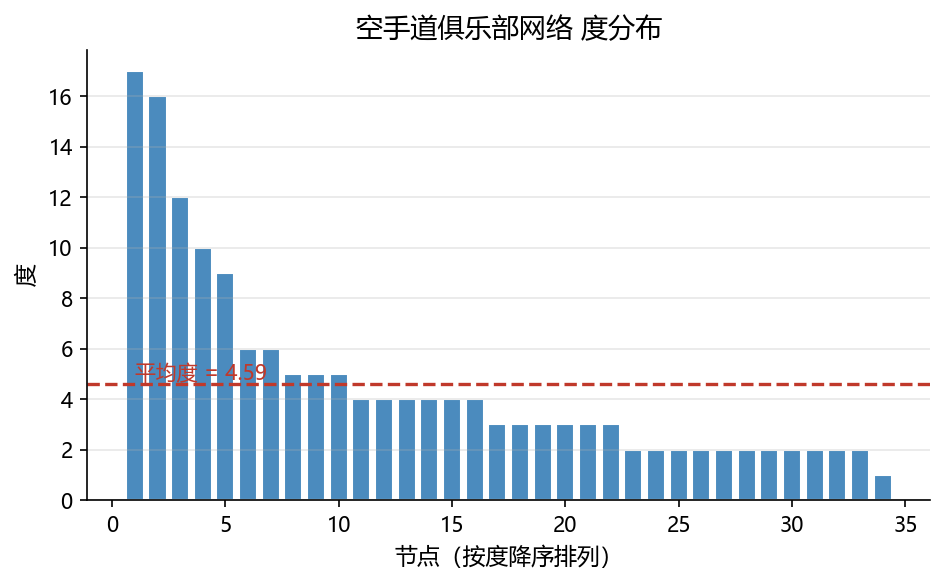
\includegraphics[keepaspectratio,alt={空手道俱乐部 度分布}]{figures/06-networkx/network_case_degree_dist.png}}
\caption{空手道俱乐部 度分布}
\end{figure}

\subsubsection{3) 全局指标}\label{ux5168ux5c40ux6307ux6807}

\begin{Shaded}
\begin{Highlighting}[]
\BuiltInTok{print}\NormalTok{(}\StringTok{"平均聚类系数:"}\NormalTok{, }\BuiltInTok{round}\NormalTok{(nx.average\_clustering(K), }\DecValTok{4}\NormalTok{))}
\BuiltInTok{print}\NormalTok{(}\StringTok{"传递性:"}\NormalTok{, }\BuiltInTok{round}\NormalTok{(nx.transitivity(K), }\DecValTok{4}\NormalTok{))}
\BuiltInTok{print}\NormalTok{(}\StringTok{"平均最短路径长度:"}\NormalTok{, }\BuiltInTok{round}\NormalTok{(nx.average\_shortest\_path\_length(K), }\DecValTok{4}\NormalTok{))}
\BuiltInTok{print}\NormalTok{(}\StringTok{"直径:"}\NormalTok{, nx.diameter(K), }\StringTok{" 半径:"}\NormalTok{, nx.radius(K))}
\NormalTok{bc }\OperatorTok{=}\NormalTok{ nx.betweenness\_centrality(K)}
\NormalTok{top }\OperatorTok{=} \BuiltInTok{sorted}\NormalTok{(bc.items(), key}\OperatorTok{=}\KeywordTok{lambda}\NormalTok{ x: x[}\DecValTok{1}\NormalTok{], reverse}\OperatorTok{=}\VariableTok{True}\NormalTok{)[:}\DecValTok{3}\NormalTok{]}
\BuiltInTok{print}\NormalTok{(}\StringTok{"介数中心性最高前3:"}\NormalTok{, top)}
\end{Highlighting}
\end{Shaded}

\begin{Shaded}
\begin{Highlighting}[]
\NormalTok{平均聚类系数: 0.5706}
\NormalTok{传递性: 0.2557}
\NormalTok{平均最短路径长度: 2.4082}
\NormalTok{直径: 5  半径: 3}
\NormalTok{介数中心性最高前3: [(0, 0.4376), (33, 0.3041), (32, 0.1452)]}
\end{Highlighting}
\end{Shaded}

解读：平均聚类系数较高（0.57），说明``朋友的朋友多是朋友''；但平均最短路径只有
2.41，直径 5，呈现``高聚类 + 短路径''的小世界特征。节点 0 与 33
的介数中心性最高，它们是连接两派之间的``桥梁''。

\subsubsection{4)
社区划分与模块度}\label{ux793eux533aux5212ux5206ux4e0eux6a21ux5757ux5ea6-1}

\begin{Shaded}
\begin{Highlighting}[]
\NormalTok{comms }\OperatorTok{=}\NormalTok{ nxcom.greedy\_modularity\_communities(K)}
\NormalTok{Q }\OperatorTok{=}\NormalTok{ modularity(K, comms)}
\BuiltInTok{print}\NormalTok{(}\StringTok{"社区个数:"}\NormalTok{, }\BuiltInTok{len}\NormalTok{(comms))}
\BuiltInTok{print}\NormalTok{(}\StringTok{"各社区大小:"}\NormalTok{, [}\BuiltInTok{len}\NormalTok{(c) }\ControlFlowTok{for}\NormalTok{ c }\KeywordTok{in}\NormalTok{ comms])}
\BuiltInTok{print}\NormalTok{(}\StringTok{"模块度 Q:"}\NormalTok{, }\BuiltInTok{round}\NormalTok{(Q, }\DecValTok{4}\NormalTok{))}
\end{Highlighting}
\end{Shaded}

\begin{Shaded}
\begin{Highlighting}[]
\NormalTok{社区个数: 3}
\NormalTok{各社区大小: [17, 9, 8]}
\NormalTok{模块度 Q: 0.411}
\end{Highlighting}
\end{Shaded}

Q≈0.41 表示网络存在较明显的社区结构；社区大小
17、9、8，且第一个社区节点编号整体偏大（8,14,15,\ldots,33），与裁判/教练两派吻合。

\subsubsection{5) 最短路径}\label{ux6700ux77edux8defux5f84}

\begin{Shaded}
\begin{Highlighting}[]
\NormalTok{path }\OperatorTok{=}\NormalTok{ nx.shortest\_path(K, source}\OperatorTok{=}\DecValTok{0}\NormalTok{, target}\OperatorTok{=}\DecValTok{33}\NormalTok{)}
\BuiltInTok{print}\NormalTok{(}\StringTok{"0 号到 33 号的最短路径:"}\NormalTok{, path)}
\BuiltInTok{print}\NormalTok{(}\StringTok{"路径长度(边数):"}\NormalTok{, nx.shortest\_path\_length(K, }\DecValTok{0}\NormalTok{, }\DecValTok{33}\NormalTok{))}
\end{Highlighting}
\end{Shaded}

\begin{Shaded}
\begin{Highlighting}[]
\NormalTok{0 号到 33 号的最短路径: [0, 8, 33]}
\NormalTok{路径长度(边数): 2}
\end{Highlighting}
\end{Shaded}

\subsubsection{6) 社区 +
路径可视化}\label{ux793eux533a-ux8defux5f84ux53efux89c6ux5316}

\begin{Shaded}
\begin{Highlighting}[]
\NormalTok{node\_color }\OperatorTok{=}\NormalTok{ \{\}}
\NormalTok{colors }\OperatorTok{=}\NormalTok{ [}\StringTok{"\#4b8bbe"}\NormalTok{, }\StringTok{"\#e07b39"}\NormalTok{, }\StringTok{"\#3a8f4f"}\NormalTok{, }\StringTok{"\#7f5fb5"}\NormalTok{, }\StringTok{"\#c0392b"}\NormalTok{]}
\ControlFlowTok{for}\NormalTok{ ci, cset }\KeywordTok{in} \BuiltInTok{enumerate}\NormalTok{(comms):}
    \ControlFlowTok{for}\NormalTok{ n }\KeywordTok{in}\NormalTok{ cset:}
\NormalTok{        node\_color[n] }\OperatorTok{=}\NormalTok{ colors[ci }\OperatorTok{\%} \BuiltInTok{len}\NormalTok{(colors)]}

\NormalTok{path\_edges }\OperatorTok{=} \BuiltInTok{list}\NormalTok{(}\BuiltInTok{zip}\NormalTok{(path[:}\OperatorTok{{-}}\DecValTok{1}\NormalTok{], path[}\DecValTok{1}\NormalTok{:]))}
\NormalTok{pos }\OperatorTok{=}\NormalTok{ nx.spring\_layout(K, seed}\OperatorTok{=}\DecValTok{42}\NormalTok{)}

\ImportTok{import}\NormalTok{ os}
\NormalTok{plt.rcParams[}\StringTok{"font.sans{-}serif"}\NormalTok{] }\OperatorTok{=}\NormalTok{ [}\StringTok{"Microsoft YaHei"}\NormalTok{, }\StringTok{"SimHei"}\NormalTok{, }\StringTok{"DejaVu Sans"}\NormalTok{]}
\NormalTok{plt.rcParams[}\StringTok{"axes.unicode\_minus"}\NormalTok{] }\OperatorTok{=} \VariableTok{False}
\NormalTok{plt.figure(figsize}\OperatorTok{=}\NormalTok{(}\FloatTok{8.2}\NormalTok{, }\FloatTok{6.2}\NormalTok{))}
\NormalTok{os.makedirs(}\StringTok{"images"}\NormalTok{, exist\_ok}\OperatorTok{=}\VariableTok{True}\NormalTok{)}
\NormalTok{nx.draw\_networkx\_edges(K, pos, alpha}\OperatorTok{=}\FloatTok{0.35}\NormalTok{, edge\_color}\OperatorTok{=}\StringTok{"\#999999"}\NormalTok{, width}\OperatorTok{=}\FloatTok{1.0}\NormalTok{)}
\NormalTok{nx.draw\_networkx\_edges(K, pos, edgelist}\OperatorTok{=}\NormalTok{path\_edges, edge\_color}\OperatorTok{=}\StringTok{"\#c0392b"}\NormalTok{, width}\OperatorTok{=}\FloatTok{3.0}\NormalTok{)}
\NormalTok{nx.draw\_networkx\_nodes(K, pos, node\_size}\OperatorTok{=}\DecValTok{260}\NormalTok{,}
\NormalTok{                       node\_color}\OperatorTok{=}\NormalTok{[node\_color[n] }\ControlFlowTok{for}\NormalTok{ n }\KeywordTok{in}\NormalTok{ K.nodes()],}
\NormalTok{                       edgecolors}\OperatorTok{=}\StringTok{"white"}\NormalTok{, linewidths}\OperatorTok{=}\FloatTok{1.2}\NormalTok{)}
\NormalTok{nx.draw\_networkx\_labels(K, pos, \{n: }\BuiltInTok{str}\NormalTok{(n) }\ControlFlowTok{for}\NormalTok{ n }\KeywordTok{in}\NormalTok{ K.nodes()\}, font\_size}\OperatorTok{=}\DecValTok{8}\NormalTok{)}
\NormalTok{plt.title(}\StringTok{"空手道俱乐部：社区划分 + 0→33 最短路径（红色）"}\NormalTok{)}
\NormalTok{plt.axis(}\StringTok{"off"}\NormalTok{)}
\NormalTok{plt.tight\_layout()}\OperatorTok{;}\NormalTok{ plt.savefig(}\StringTok{"figures/06{-}networkx/network\_case\_communities.png"}\NormalTok{)}
\BuiltInTok{print}\NormalTok{(}\StringTok{"已保存 communities"}\NormalTok{)}
\end{Highlighting}
\end{Shaded}

\begin{figure}
\centering
\pandocbounded{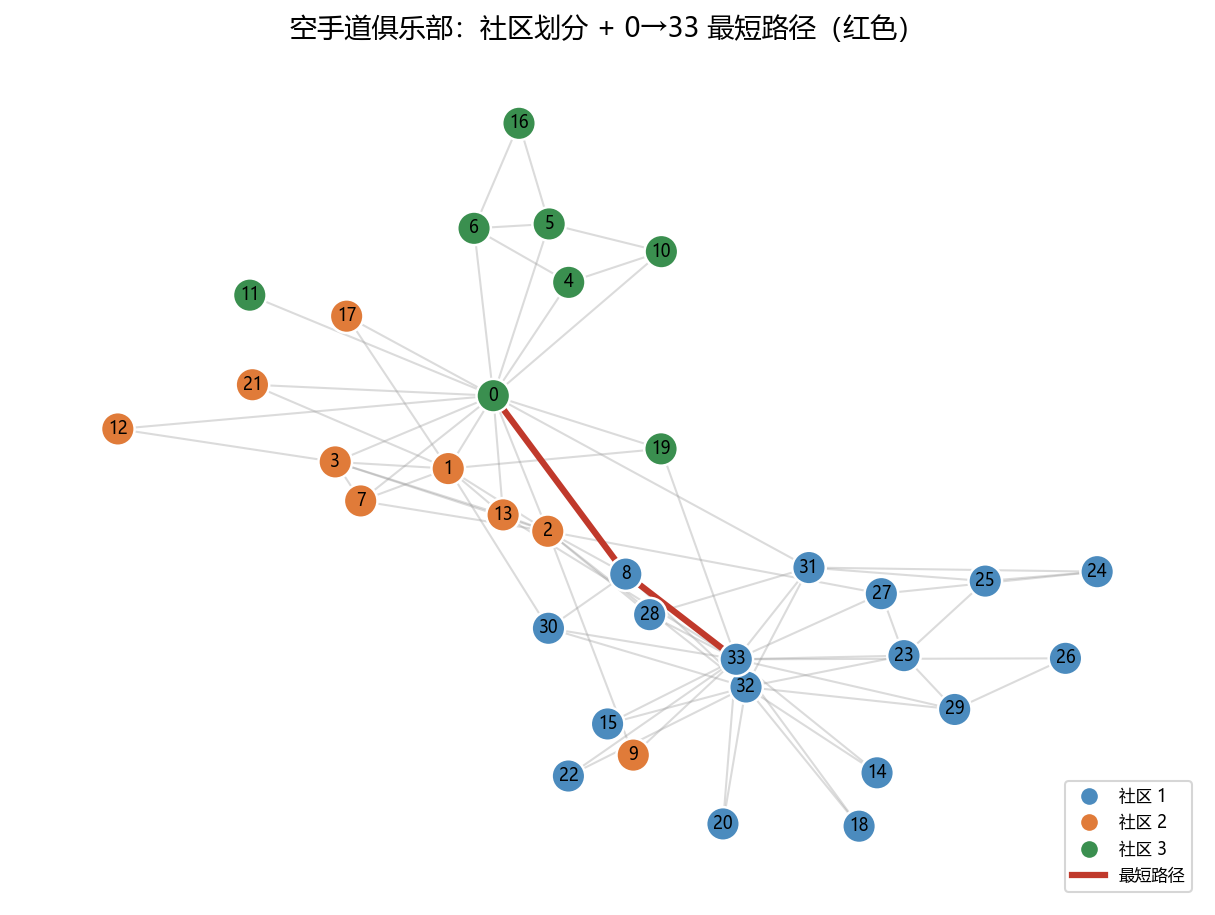
\includegraphics[keepaspectratio,alt={空手道俱乐部 社区划分与最短路径}]{figures/06-networkx/network_case_communities.png}}
\caption{空手道俱乐部 社区划分与最短路径}
\end{figure}

\subsubsection{主要用法 / API}\label{ux4e3bux8981ux7528ux6cd5-api-27}

{\def\LTcaptype{none} % do not increment counter
\begin{longtable}[]{@{}
  >{\raggedright\arraybackslash}p{(\linewidth - 4\tabcolsep) * \real{0.3333}}
  >{\raggedright\arraybackslash}p{(\linewidth - 4\tabcolsep) * \real{0.3333}}
  >{\raggedright\arraybackslash}p{(\linewidth - 4\tabcolsep) * \real{0.3333}}@{}}
\toprule\noalign{}
\begin{minipage}[b]{\linewidth}\raggedright
需求
\end{minipage} & \begin{minipage}[b]{\linewidth}\raggedright
写法
\end{minipage} & \begin{minipage}[b]{\linewidth}\raggedright
说明
\end{minipage} \\
\midrule\noalign{}
\endhead
\bottomrule\noalign{}
\endlastfoot
载入经典网络 & \texttt{nx.karate\_club\_graph()} & 34 节点 78 边 \\
度分布 &
\texttt{sorted({[}d\ for\ \_,\ d\ in\ K.degree(){]},\ reverse=True)} &
长尾/无标度特征 \\
全局指标 & \texttt{nx.average\_clustering} / \texttt{nx.transitivity} /
\texttt{nx.average\_shortest\_path\_length} & 小世界效应 \\
社区划分 & \texttt{nxcom.greedy\_modularity\_communities(K)} &
返回社区集合 \\
模块度 & \texttt{modularity(K,\ comms)} & 划分质量 Q \\
最短路径 & \texttt{nx.shortest\_path(K,\ 0,\ 33)} & 无权最短路 \\
可视化 & \texttt{nx.draw\_networkx\_*} +
\texttt{spring\_layout(K,\ seed=42)} & 固定布局便于复现 \\
\end{longtable}
}

\subsubsection{常见错误}\label{ux5e38ux89c1ux9519ux8bef-27}

\begin{enumerate}
\def\labelenumi{\arabic{enumi}.}
\tightlist
\item
  忘记导入社区子模块：社区函数在 \texttt{networkx.algorithms.community}
  下，需要
  \texttt{from\ networkx.algorithms\ import\ community\ as\ nxcom}。
\item
  把模块度 Q 当成``越大越绝对正确''：Q 是相对指标，0.41 对 34
  节点网络已算不错，但不同算法或 seed 可能得到不同社区数。
\item
  \texttt{spring\_layout} 不传
  \texttt{seed}：每次布局不同，截图/复现对不上。
\item
  把``度分布降序图''误当成直方图：这里 x
  轴是``按度排序的节点编号''，并不是度数分箱。
\end{enumerate}

\subsubsection{拓展 / 跟练}\label{ux62d3ux5c55-ux8ddfux7ec3-15}

\begin{enumerate}
\def\labelenumi{\arabic{enumi}.}
\tightlist
\item
  分别计算 0 号与 33
  号的度、介数中心性、接近中心性，比较两者谁更像``中心''。
\item
  用 \texttt{nx.community.louvain\_communities(K,\ seed=42)}
  划分，比较社区个数与 Q 值。
\item
  把``0→33
  最短路径''推广成``所有点对平均最短路径''，并解释``六度分隔''。
\item
  用 \texttt{nx.to\_numpy\_array(K)} 得到 34x34
  邻接矩阵，验证对称；再交给 SciPy 做特征值（可选）。
\end{enumerate}

\begin{center}\rule{0.5\linewidth}{0.5pt}\end{center}

\subsection{案例结论}\label{ux6848ux4f8bux7ed3ux8bba}

\begin{itemize}
\tightlist
\item
  度分布有明显``长尾''：少数节点度很高（节点 0
  度=17），符合社交网络的无标度特征；
\item
  高聚类系数、短平均路径，说明该网络具有小世界效应；
\item
  社区检测给出 3 个社区、Q≈0.41，划分质量较好；
\item
  最短路径 0→8→33
  表明两位``领袖''其实只隔一个中间人，再次体现``六度分隔''。
\end{itemize}

\subsection{拓展任务}\label{ux62d3ux5c55ux4efbux52a1-6}

\begin{enumerate}
\def\labelenumi{\arabic{enumi}.}
\tightlist
\item
  分别计算 0 号与 33
  号节点的度、介数中心性、接近中心性，比较两者谁更像``中心''；
\item
  修改 seed 重新布局，观察社区/路径是否变化（应不变，因为 graph
  本身不变，只有节点画的位置变）；
\item
  用 nx.connected\_components
  检查该网络是否连通；若不连通，找出孤立分量；
\item
  用
  louvain\_communities（networkx.algorithms.community.louvain\_communities）划分，比较社区个数与
  Q 值。
\end{enumerate}

\subsection{本章综合练习（上机任务）}\label{ux672cux7ae0ux7efcux5408ux7ec3ux4e60ux4e0aux673aux4efbux52a1-2}

\begin{enumerate}
\def\labelenumi{\arabic{enumi}.}
\tightlist
\item
  用 erdos\_renyi\_graph(100, 0.05, seed=1)
  生成随机网络，计算平均聚类系数与平均最短路径，与 karate
  网络对比，说明``小世界''差异；
\item
  在 karate\_club\_graph 上分别计算 average\_clustering 与
  transitivity，并解释两者为何不同；
\item
  把本案例整理成一个 .ipynb，写出 3 句结论。
\end{enumerate}

\subsection{延伸阅读}\label{ux5ef6ux4f38ux9605ux8bfb-29}

\begin{itemize}
\tightlist
\item
  Zachary
  空手道俱乐部数据集说明：\href{https://networkx.org/documentation/stable/reference/generated/networkx.generators.social.karate_club_graph.html}{链接}
\item
  NetworkX
  社区检测模块：\href{https://networkx.org/documentation/stable/reference/algorithms/community.html}{链接}
\item
  NetworkX
  布局算法：\href{https://networkx.org/documentation/stable/reference/drawing.html}{链接}
\end{itemize}

\section{05
常见误区与技巧}\label{ux5e38ux89c1ux8befux533aux4e0eux6280ux5de7-5}

\begin{quote}
本章为新增``查漏补缺''页：把学生最容易踩的坑集中列出，并给出正确写法与性能/调试技巧。
\end{quote}

\subsection{1.
高频误区速查表}\label{ux9ad8ux9891ux8befux533aux901fux67e5ux8868-5}

{\def\LTcaptype{none} % do not increment counter
\begin{longtable}[]{@{}
  >{\raggedright\arraybackslash}p{(\linewidth - 6\tabcolsep) * \real{0.2500}}
  >{\raggedright\arraybackslash}p{(\linewidth - 6\tabcolsep) * \real{0.2500}}
  >{\raggedright\arraybackslash}p{(\linewidth - 6\tabcolsep) * \real{0.2500}}
  >{\raggedright\arraybackslash}p{(\linewidth - 6\tabcolsep) * \real{0.2500}}@{}}
\toprule\noalign{}
\begin{minipage}[b]{\linewidth}\raggedright
\#
\end{minipage} & \begin{minipage}[b]{\linewidth}\raggedright
误区 / 错误写法
\end{minipage} & \begin{minipage}[b]{\linewidth}\raggedright
正确做法
\end{minipage} & \begin{minipage}[b]{\linewidth}\raggedright
原因
\end{minipage} \\
\midrule\noalign{}
\endhead
\bottomrule\noalign{}
\endlastfoot
1 & 把 G.nodes() / G.edges() 当普通列表直接修改 & 用 list(G.nodes())
转列表；改图用 add\_node / remove\_node & 返回的是视图对象 \\
2 & 在有向图上用 G.neighbors(2) 当``指向 2 的节点'' & 用
DG.predecessors(2) 找前驱，DG.successors(2) 找后继 & 邻居 = 后继 \\
3 & zip(G.nodes(), G.in\_degree(), G.out\_degree()) 解包 & 用
dict(DG.in\_degree()) 或 DG.in\_degree(node) & in\_degree 返回 (节点,
度数) 对 \\
4 & add\_edge(u, v, 10) 当权重 & add\_weighted\_edges\_from 或
add\_edge(u, v, weight=10) & 三参数不是权重签名 \\
5 & 随机图不设 seed & nx.erdos\_renyi\_graph(10, 0.3, seed=42) &
结果不可复现 \\
6 & 把 average\_shortest\_path\_length 用在``有权图''上却不带 weight &
加 weight=``weight'' 参数；无权图则默认 & 默认按无权（每条边=1）计算 \\
7 & 用 Dijkstra 处理负权边 & 改用 bellman\_ford\_path / floyd\_warshall
& Dijkstra 依赖非负权 \\
8 & 在``数三角形/算模块度''时以为结果为整数 & triangles 是
dict，总三角形数 = sum//3；模块度 Q 是 float & 不同数值语义 \\
9 & 认为 minimum\_spanning\_tree 结论就是``最短路径'' &
分清``连通所有点总权重最小''与``两点间距离最小'' & 目标不同 \\
10 & 用 nx.diameter 对不连通图 & 先判断
is\_connected，或按连通分量分别算 & 不连通无有限直径 \\
11 & 用 nx.to\_numpy\_array 得到的是 float 矩阵 & 需要整数可转
A.astype(int) & 默认 float64 \\
12 & 社区检测结果当成唯一正确解 & 多算法多 seed 交叉验证，报告 Q
值而非``社区是\ldots\ldots'' & 社区划分非唯一 \\
\end{longtable}
}

\subsection{2. 原理级注意点}\label{ux539fux7406ux7ea7ux6ce8ux610fux70b9}

\subsubsection{2.1 视图 vs
数据结构}\label{ux89c6ux56fe-vs-ux6570ux636eux7ed3ux6784}

G.nodes() 与 G.edges()
是视图对象，支持迭代与成员判断，但不支持``直接赋值''。要得到稳定快照用：

\begin{Shaded}
\begin{Highlighting}[]
\ImportTok{import}\NormalTok{ networkx }\ImportTok{as}\NormalTok{ nx}
\NormalTok{G }\OperatorTok{=}\NormalTok{ nx.Graph()}
\NormalTok{G.add\_edges\_from([(}\DecValTok{1}\NormalTok{, }\DecValTok{2}\NormalTok{), (}\DecValTok{2}\NormalTok{, }\DecValTok{3}\NormalTok{)])}

\NormalTok{node\_list }\OperatorTok{=} \BuiltInTok{list}\NormalTok{(G.nodes())}
\NormalTok{edge\_list }\OperatorTok{=} \BuiltInTok{list}\NormalTok{(G.edges())}
\NormalTok{degree\_view }\OperatorTok{=} \BuiltInTok{dict}\NormalTok{(G.degree())}
\BuiltInTok{print}\NormalTok{(node\_list, edge\_list, degree\_view)}
\end{Highlighting}
\end{Shaded}

\subsubsection{2.2
有向图连通性的``方向坑''}\label{ux6709ux5411ux56feux8fdeux901aux6027ux7684ux65b9ux5411ux5751}

有向图的 is\_connected 不存在；要用 is\_strongly\_connected 与
is\_weakly\_connected。把无向图用 nx.DiGraph(G)
转换后，每条无向边会变成双向两条边，所以结论可能与你直觉不同。

\subsubsection{2.3 加权 vs 无权}\label{ux52a0ux6743-vs-ux65e0ux6743}

大多网络函数默认按``无权''处理（每条边权重=1）。一旦图带 weight
属性，要么显式传
weight=``weight''，要么接受默认``无权''结果。二者结果可能完全不同。

\subsection{3. 性能技巧}\label{ux6027ux80fdux6280ux5de7-4}

\begin{itemize}
\tightlist
\item
  \textbf{用生成器造图}：path\_graph / cycle\_graph /
  erdos\_renyi\_graph 比手动 add\_node 循环快得多；
\item
  \textbf{批量加边}：add\_edges\_from /
  add\_weighted\_edges\_from，不要一条条 add\_edge；
\item
  \textbf{中心性按需计算}：betweenness\_centrality
  默认精确算法在大图很慢；可用 k 参数（k
  个随机源）近似，或只计算关心的节点子集；
\item
  \textbf{社区检测选算法}：greedy\_modularity\_communities
  适合中等规模；超大图可用 louvain\_communities（更快）；
\item
  \textbf{复用图对象}：对同一张图反复调用算法时，先复制为
  G.copy()，避免原地修改影响后续分析；
\item
  \textbf{大图用稀疏结构}：需要把邻接矩阵交给 SciPy 时，用
  nx.to\_scipy\_sparse\_array(G) 得到稀疏矩阵，节省内存（若安装了
  scipy）。
\end{itemize}

\subsection{4. 调试建议}\label{ux8c03ux8bd5ux5efaux8bae-5}

\begin{enumerate}
\def\labelenumi{\arabic{enumi}.}
\tightlist
\item
  先打印 G.number\_of\_nodes()、G.number\_of\_edges()，确认图建对了；
\item
  用 sorted(G.nodes()) 检查节点是否被意外``自动补全''；
\item
  报路径错误时先判断连通性：\texttt{nx.is\_connected(G)}（有向用
  \texttt{is\_strongly\_connected}）；
\item
  带权问题先把边打印出来：\texttt{G.edges(data=True)}，确认 weight
  属性名与数值；
\item
  较慢的算法先在小图上验证（如 path\_graph(10)）再加到大数据；
\item
  绘图布局不稳定时，给 spring\_layout 传 seed，便于复现。
\end{enumerate}

\subsection{5.
本章小结（自测）}\label{ux672cux7ae0ux5c0fux7ed3ux81eaux6d4b-3}

\begin{itemize}
\tightlist
\item[$\square$]
  能区分 Graph 与 DiGraph，说出 neighbors / predecessors / successors
  的差异；
\item[$\square$]
  能给图加节点属性、边权重，并用 nodes(data=True)、edges(data=True)
  查看；
\item[$\square$]
  能说出度/度分布、聚类系数、传递性、介数中心性、接近中心性、模块度的含义；
\item[$\square$]
  能根据图特性为最短路径选择 Dijkstra / Bellman-Ford / Floyd-Warshall；
\item[$\square$]
  能用 minimum\_spanning\_tree 求 MST 并算总权重；
\item[$\square$]
  能完成 04 综合案例并在图上可视化社区与最短路径。
\end{itemize}

\subsection{延伸阅读}\label{ux5ef6ux4f38ux9605ux8bfb-30}

\begin{itemize}
\tightlist
\item
  NetworkX
  官方``算法总览''：\href{https://networkx.org/documentation/stable/reference/algorithms/index.html}{链接}
\item
  NetworkX
  官方绘图指南：\href{https://networkx.org/documentation/stable/reference/drawing.html}{链接}
\item
  NetworkX
  官方``性能提示''与稀疏表示：\href{https://networkx.org/documentation/stable/reference/convert.html}{链接}
\end{itemize}

\newpage
